\documentclass[12pt,a4paper]{article}

% =====================================================================
% CẤU HÌNH GÓI & ĐỊNH DẠNG TƯƠNG THÍCH ĐA TRÌNH BIÊN DỊCH (OVERLEAF / LOCAL)
% Hỗ trợ tự động cả pdfLaTeX, XeLaTeX và LuaLaTeX
% =====================================================================
\usepackage{iftex}
\ifPDFTeX
  \usepackage[utf8]{inputenc}
  \usepackage[vietnamese]{babel}
  \usepackage[T5,T1]{fontenc}
  \usepackage{lmodern}
\else
  \usepackage{fontspec}
  \usepackage{polyglossia}
  \setdefaultlanguage{vietnamese}
\fi

\usepackage[a4paper,margin=2cm,top=2.5cm,bottom=2.5cm]{geometry}
\usepackage{amsmath,amssymb,amsfonts,mathtools}
\usepackage{graphicx}
\usepackage{float}
\usepackage{booktabs}
\usepackage{tabularx}
\usepackage{array}
\usepackage{multirow}
\usepackage{colortbl}
\usepackage{xcolor}
\usepackage{caption}
\usepackage{subcaption}
\usepackage{fancyhdr}
\usepackage{titlesec}
\usepackage{algorithm}
\usepackage{algpseudocode}
\usepackage{listings}
\usepackage{tikz}
\usetikzlibrary{shapes.geometric, arrows, positioning}

% Đường dẫn tìm kiếm ảnh (tự động nhận diện khi biên dịch tại thư mục gốc hoặc thư mục con)
\graphicspath{{./}{outputs/}{Student-Performance-Decision-Tree/outputs/}}

% Bảng màu học thuật chuẩn
\definecolor{primaryblue}{RGB}{41, 128, 185}
\definecolor{darkblue}{RGB}{26, 82, 118}
\definecolor{headerblue}{RGB}{235, 245, 251}
\definecolor{codegreen}{RGB}{39, 174, 96}
\definecolor{codegray}{RGB}{127, 140, 141}
\definecolor{codepurple}{RGB}{142, 68, 173}
\definecolor{backcolour}{RGB}{248, 249, 250}

% Cấu hình hyperlink
\usepackage{hyperref}
\hypersetup{
    colorlinks=true,
    linkcolor=primaryblue,
    filecolor=darkblue,
    urlcolor=primaryblue,
    citecolor=darkblue,
    pdftitle={Báo Cáo Bài Tập Lớn Cá Nhân: Dự Đoán Sớm Kết Quả Học Tập Sinh Viên Bằng Decision Tree},
    pdfauthor={Sinh Viên HaUI},
    pdfsubject={Khai Phá Dữ Liệu / Học Máy}
}

% Cấu hình hiển thị code Python
\lstdefinestyle{pythonstyle}{
    backgroundcolor=\color{backcolour},   
    commentstyle=\color{codegreen}\itshape,
    keywordstyle=\color{primaryblue}\bfseries,
    numberstyle=\tiny\color{codegray},
    stringstyle=\color{codepurple},
    basicstyle=\ttfamily\footnotesize,
    breakatwhitespace=false,         
    breaklines=true,                 
    captionpos=b,                    
    keepspaces=true,                 
    numbers=left,                    
    numbersep=5pt,                  
    showspaces=false,                
    showstringspaces=false,
    showtabs=false,                  
    tabsize=4,
    frame=single,
    rulecolor=\color{codegray!30}
}
\lstset{style=pythonstyle}

% Cấu hình Header & Footer
\pagestyle{fancy}
\fancyhf{}
\fancyhead[L]{\fontsize{9}{11}\selectfont\textit{Học phần Khai phá Dữ liệu --- Báo cáo Bài tập lớn}}
\fancyhead[R]{\fontsize{9}{11}\selectfont\textit{Dự đoán sớm bằng Decision Tree}}
\fancyfoot[C]{\thepage}
\renewcommand{\headrulewidth}{0.4pt}
\renewcommand{\footrulewidth}{0.4pt}

% Giãn dòng
\renewcommand{\baselinestretch}{1.25}
\setlength{\parskip}{6pt}

% =====================================================================
% BẮT ĐẦU TÀI LIỆU
% =====================================================================
\begin{document}

% -------------------------------------------------------------
% TRANG BÌA CHUẨN ĐẠI HỌC CÔNG NGHIỆP HÀ NỘI
% -------------------------------------------------------------
\begin{titlepage}
    \begin{center}
        \textbf{\large BỘ GIÁO DỤC VÀ ĐÀO TẠO}\\[0.2cm]
        \textbf{\large TRƯỜNG ĐẠI HỌC CÔNG NGHIỆP HÀ NỘI}\\[0.2cm]
        \textbf{\large KHOA CÔNG NGHỆ THÔNG TIN}\\[0.3cm]
        \rule{0.6\textwidth}{1.5pt}\\[2.0cm]

        \textbf{\Large BÁO CÁO BÀI TẬP LỚN CÁ NHÂN}\\[0.3cm]
        \textbf{\large HỌC PHẦN: KHAI PHÁ DỮ LIỆU / HỌC MÁY}\\[1.5cm]

        \begin{minipage}{0.9\textwidth}
            \centering
            \textbf{\huge\color{primaryblue} DỰ ĐOÁN SỚM KẾT QUẢ HỌC TẬP CỦA SINH VIÊN BẰNG THUẬT TOÁN DECISION TREE}\\[0.5cm]
            \textit{\large Ứng dụng trên tập dữ liệu hồ sơ học tập 1.656 sinh viên với giao thức Zero Label Leakage và 5-Fold Stratified Cross-Validation}
        \end{minipage}\\[2.5cm]

        \begin{minipage}{0.85\textwidth}
            \large
            \begin{tabular}{ll}
                \textbf{Sinh viên thực hiện:} & \dotfill \\
                \textbf{Mã số sinh viên (MSSV):} & \dotfill \\
                \textbf{Lớp sinh hoạt:} & \dotfill \\
                \textbf{Hệ số đóng góp:} & \textbf{1.0 (100\% --- Nghiên cứu độc lập)} \\[0.4cm]
                \textbf{Giảng viên phụ trách:} & Bộ môn Khai phá Dữ liệu \\
                \textbf{Khoa:} & Công nghệ Thông tin
            \end{tabular}
        \end{minipage}\\[2.5cm]

        \vfill
        \textbf{\large HÀ NỘI --- NĂM HỌC 2026}
    \end{center}
\end{titlepage}

% -------------------------------------------------------------
% TRANG BẢNG ĐÓNG GÓP & LỜI CAM ĐOAN
% -------------------------------------------------------------
\newpage
\thispagestyle{plain}
\begin{center}
    \section*{THÔNG TIN SINH VIÊN & BẢNG CAM ĐOAN ĐÓNG GÓP}
\end{center}
\addcontentsline{toc}{section}{Thông tin sinh viên \& Bảng cam đoan đóng góp}

Căn cứ vào quy chế đánh giá học phần Khai phá Dữ liệu: Điểm bài viết báo cáo kỹ thuật (trọng số 50\%) và điểm vấn đáp/thuyết trình (trọng số 50\%) được chấm trực tiếp cho cá nhân sinh viên thực hiện độc lập đề tài:

\begin{table}[H]
\centering
\begin{tabularx}{\textwidth}{|c|X|c|c|X|c|}
\hline
\rowcolor{primaryblue}
\textbf{\color{white}STT} & \textbf{\color{white}Họ và Tên Sinh Viên} & \textbf{\color{white}Mã Sinh Viên} & \textbf{\color{white}Lớp} & \textbf{\color{white}Nhiệm Vụ Thực Hiện Toàn Trình} & \textbf{\color{white}Hệ Số} \\
\hline
1 & \dotfill & \dotfill & \dotfill & \textbf{Thực hiện độc lập 100\%:} Khảo sát tập dữ liệu 1.656 sinh viên, thiết kế pipeline tiền xử lý, huấn luyện Decision Tree và mô hình đối chứng Logistic Regression, kiểm định chéo 5-Fold Stratified CV, xuất toàn bộ 5 biểu đồ thực nghiệm 300 DPI và viết báo cáo khoa học hoàn chỉnh. & \textbf{1.0 (100\%)} \\
\hline
\end{tabularx}
\caption{Bảng xác nhận mức độ đóng góp cá nhân thực hiện đề tài}
\end{table}

\vspace{1.5cm}
\noindent\textbf{Lời cam đoan của sinh viên:}
\begin{quote}
\textit{Tôi xin cam đoan đây là công trình bài tập lớn do bản thân tôi tự nghiên cứu, lập trình và hoàn thiện độc lập. Mọi số liệu thực nghiệm, bảng biểu đối sánh và đồ thị minh họa trong báo cáo đều được trích xuất trung thực từ mã nguồn chương trình thực thi (\texttt{main.py}), bộ dữ liệu sử dụng đã được khử định danh học thuật và tuân thủ các chuẩn mực nghiên cứu khoa học. Tôi xin hoàn toàn chịu trách nhiệm trước Bộ môn và Khoa về tính trung thực của báo cáo này.}
\end{quote}

\vspace{2cm}
\begin{flushright}
    \textit{Hà Nội, ngày \dots\dots\ tháng \dots\dots\ năm 2026}\\[0.2cm]
    \textbf{Sinh viên thực hiện đề tài}\\[2.5cm]
    \textbf{(Ký và ghi rõ họ tên)}
\end{flushright}

% -------------------------------------------------------------
% MỤC LỤC TỰ ĐỘNG
% -------------------------------------------------------------
\newpage
\tableofcontents
\newpage
\listoftables
\listoffigures

\newpage

% =====================================================================
% PHẦN I: BÁO CÁO HỌC THUẬT (5 CHƯƠNG)
% =====================================================================
\part{BÁO CÁO KỸ THUẬT CHUẨN ĐỀ CƯƠNG (5 CHƯƠNG)}

\section{GIỚI THIỆU TỔNG QUAN}

\subsection{Bối Cảnh Bài Toán \& Tính Cấp Thiết}
Trong các cơ sở giáo dục đại học đào tạo theo học chế tín chỉ, sinh viên năm thứ nhất thường phải đối mặt với bước chuyển tiếp rất lớn về phương pháp tiếp cận kiến thức, tính chủ động tự học và cường độ làm việc. Việc gặp bỡ ngỡ trước khối lượng kiến thức khoa học cơ bản (Giải tích, Vật lý đại cương) và kỹ thuật cơ sở thường dẫn đến tình trạng sa sút kết quả học tập, bị cảnh báo học vụ hoặc thậm chí bị buộc thôi học ở các học kỳ sau.

Do đó, bài toán \textbf{Khai phá Dữ liệu Giáo dục (Educational Data Mining --- EDM)} nhằm xây dựng \textbf{Hệ thống cảnh báo sớm (Early Warning System)} mang ý nghĩa thực tiễn to lớn: giúp nhà trường và đội ngũ cố vấn học tập chủ động phát hiện sớm sinh viên có nguy cơ sa sút để can thiệp, tư vấn và hỗ trợ phương pháp học tập ngay sau năm nhất, thay vì chờ đến khi kết quả đã an bài ở năm cuối.

\subsection{Mục Tiêu \& Phạm Vi Đề Tài}
Đề tài tập trung giải quyết bài toán phân lớp nhị phân kết quả học tập tốt nghiệp của sinh viên đại học. Mục tiêu và phạm vi cụ thể gồm:
\begin{enumerate}
    \item Khảo sát hiện trạng phân bố điểm tích lũy GPA toàn khóa và sự tương quan giữa các môn học Năm 1 với năng lực tốt nghiệp của sinh viên.
    \item Ứng dụng thuật toán \textbf{Cây quyết định (Decision Tree Classifier)} để dự đoán sớm sinh viên sẽ đạt loại \textbf{Khá/Giỏi} ($\text{GPA} \ge 2.50$) hay \textbf{Trung bình/Yếu} ($\text{GPA} < 2.50$) chỉ bằng kết quả các môn học của Năm thứ nhất (15 môn học nền tảng).
    \item Đảm bảo tính minh bạch và khả năng giải thích (\textit{Interpretability}) của mô hình cây thông qua việc trực quan hóa các quy tắc rẽ nhánh (\textit{If-Then rules}) và xếp hạng các môn học có ảnh hưởng lớn nhất.
    \item Tuân thủ nghiêm ngặt nguyên tắc \textbf{Zero Data Leakage}: Không sử dụng điểm của các năm học sau hoặc các thông tin rò rỉ nhãn vào quá trình dự đoán sớm.
\end{enumerate}

\subsection{Tổng Quan Machine Learning \& Bài Toán Muốn Làm}
\textit{Học máy (Machine Learning) là lĩnh vực trí tuệ nhân tạo nghiên cứu các thuật toán cho phép máy tính tự động đúc kết quy luật từ dữ liệu quá khứ. Trong bài toán phân lớp kết quả học tập này, tác giả lựa chọn thuật toán Cây quyết định (Decision Tree Classifier) với tiêu chí Độ vấy bẩn Gini (Gini Impurity). Lý do then chốt để lựa chọn Cây quyết định trong giáo dục là cấu trúc dạng cây phân cấp (White-box model) mang tính minh bạch tuyệt đối: cung cấp các quy tắc If-Then trực quan và các ngưỡng điểm số học cụ thể cho từng môn học, giúp cố vấn học tập dễ dàng giải thích và định hướng cho sinh viên, vượt trội hơn các mô hình hộp đen phức tạp.}

\subsection{Một Số Công Việc Liên Quan (Related Works)}
Nghiên cứu kinh điển của Cortez \& Silva (2008) \cite{cortez2008} đã mở đầu xu hướng áp dụng các thuật toán Học máy (Decision Tree, Random Forest, SVM) để dự đoán kết quả học tập, chỉ ra rằng điểm các kỳ học đầu tiên đóng vai trò quyết định trong việc định hình kết quả cuối khóa. Romero \& Ventura (2010) \cite{romero2010} đã khảo sát toàn diện các kỹ thuật khai phá dữ liệu giáo dục và nhấn mạnh rằng tính khả giải (\textit{Interpretability}) của mô hình Cây quyết định là tiêu chí hàng đầu để ứng dụng trong môi trường đào tạo. Tại Việt Nam, các nghiên cứu tại các trường kỹ thuật lớn cũng khẳng định điểm số các môn khoa học cơ bản (Giải tích, Vật lý, Ngoại ngữ) ở năm nhất có hệ số tương quan rất cao với năng lực tốt nghiệp của sinh viên.

% -------------------------------------------------------------
\newpage
\section{CƠ SỞ LÝ THUYẾT THUẬT TOÁN DECISION TREE}

\subsection{Bản Chất Của Cây Quyết Định}
Cây quyết định (Decision Tree) là phương pháp học có giám sát phi tham số (\textit{non-parametric supervised learning}). Mô hình tổ chức tri thức học được dưới dạng cấu trúc cây phân cấp bao gồm:
\begin{itemize}
    \item \textbf{Nút gốc (Root Node):} Chứa toàn bộ tập dữ liệu huấn luyện ban đầu trước khi bị phân chia.
    \item \textbf{Nút nội vi (Decision Nodes):} Biểu diễn một điều kiện kiểm tra trên một thuộc tính cụ thể (ví dụ: $\text{Điểm môn Điện - Điện tử ô tô} \le 2.25$).
    \item \textbf{Nhánh (Branches):} Tương ứng với kết quả của phép kiểm tra điều kiện (Đúng hoặc Sai).
    \item \textbf{Nút lá (Leaf Nodes):} Đại diện cho nhãn phân lớp cuối cùng (Khá-Giỏi hoặc Trung bình-Yếu) cùng phân bố xác suất tương ứng.
\end{itemize}

\subsection{Các Tiêu Chí Phân Tách Toán Học}
Để tìm thuộc tính và điểm ngưỡng phân chia tối ưu tại mỗi bước, thuật toán đánh giá mức độ thuần khiết (\textit{Purity}) của các tập con sinh ra.

\subsubsection{1. Độ vấy bẩn Gini (Gini Impurity --- Thuật toán CART)}
Đo lường xác suất một phần tử được gán nhãn ngẫu nhiên bị phân loại sai nếu nhãn được rút ngẫu nhiên theo phân bố trong tập:
\begin{equation}
    \text{Gini}(D) = 1 - \sum_{i=1}^{C} p_i^2
\end{equation}
Trong bài toán phân lớp nhị phân ($C = 2$):
\begin{itemize}
    \item $\text{Gini} = 0$: Tập dữ liệu hoàn toàn thuần khiết (100\% mẫu cùng thuộc về một nhãn).
    \item $\text{Gini} = 0.5$: Tập dữ liệu hỗn độn cực đại (50\% mẫu nhãn 0, 50\% mẫu nhãn 1).
\end{itemize}

Khi phân tách tập $D$ thành hai tập con $D_1$ và $D_2$ theo thuộc tính $A$ tại ngưỡng $\theta$, Độ vấy bẩn Gini có trọng số là:
\begin{equation}
    \text{Gini}_{\text{split}}(D, A) = \frac{|D_1|}{|D|} \text{Gini}(D_1) + \frac{|D_2|}{|D|} \text{Gini}(D_2)
\end{equation}
Thuật toán chọn thuộc tính $A^*$ và ngưỡng $\theta^*$ sao cho $\text{Gini}_{\text{split}}$ đạt giá trị \textbf{nhỏ nhất} (tương ứng với mức giảm Gini $\Delta \text{Gini}$ lớn nhất).

\subsubsection{2. Entropy và Độ lợi thông tin (Information Gain --- Thuật toán ID3/C4.5)}
Đo lường lượng thông tin bất định của tập dữ liệu:
\begin{equation}
    \text{Entropy}(D) = - \sum_{i=1}^{C} p_i \log_2(p_i)
\end{equation}
\begin{equation}
    \text{Information Gain}(D, A) = \text{Entropy}(D) - \sum_{v \in \text{Values}(A)} \frac{|D_v|}{|D|} \text{Entropy}(D_v)
\end{equation}

\subsection{Các Bước Xây Dựng Cây Quyết Định (Algorithm Steps / Pseudocode)}
Quy trình xây dựng Cây quyết định CART được thực hiện theo chiến lược đệ quy tham lam từ trên xuống (\textit{Top-down Greedy Recursion}):

\begin{algorithm}[H]
\caption{Thuật toán Xây dựng Cây Quyết định CART Phân lớp}\label{alg:cart}
\begin{algorithmic}[1]
\Require Tập dữ liệu huấn luyện $D$, danh sách thuộc tính $\mathcal{F}$, độ sâu tối đa $d_{\max}$, số mẫu lá tối thiểu $n_{\min}$
\Ensure Cây quyết định $T$
\Function{BuildTree}{$D$, $depth$}
    \If{$depth \ge d_{\max}$ \textbf{or} $|D| \le n_{\min}$ \textbf{or} $\text{Gini}(D) == 0$}
        \State \Return \Call{CreateLeafNode}{\text{MajorityClass}($D$)}
    \EndIf
    \State $(A^*, \theta^*, \text{Gini}_{\min}) \gets (\text{None}, \text{None}, +\infty)$
    \For{mỗi thuộc tính $A \in \mathcal{F}$}
        \For{mỗi ngưỡng phân chia khả dĩ $\theta \in \text{UniqueValues}(D, A)$}
            \State Chia $D$ thành $D_1 = \{x \in D \mid x_A \le \theta\}$ và $D_2 = \{x \in D \mid x_A > \theta\}$
            \State Tính $\text{Gini}_{\text{split}} = \frac{|D_1|}{|D|} \text{Gini}(D_1) + \frac{|D_2|}{|D|} \text{Gini}(D_2)$
            \If{$\text{Gini}_{\text{split}} < \text{Gini}_{\min}$}
                \State $(A^*, \theta^*, \text{Gini}_{\min}) \gets (A, \theta, \text{Gini}_{\text{split}})$
            \EndIf
        \EndFor
    \EndFor
    \State $T_{\text{left}} \gets$ \Call{BuildTree}{$D_1^*, depth + 1$}
    \State $T_{\text{right}} \gets$ \Call{BuildTree}{$D_2^*, depth + 1$}
    \State \Return \Call{CreateInternalNode}{$A^*, \theta^*, T_{\text{left}}, T_{\text{right}}$}
\EndFunction
\end{algorithmic}
\end{algorithm}

\subsection{Kỹ Thuật Kiểm Soát Quá Khớp (Pre-pruning)}
Nếu để cây phát triển tự do không kiểm soát, mô hình sẽ cố gắng phân nhánh để bao phủ từng điểm nhiễu của tập Train, dẫn đến hiện tượng \textbf{Quá khớp (Overfitting)} và làm suy giảm khả năng dự đoán trên dữ liệu mới. Đề tài áp dụng kỹ thuật \textbf{Tiền cắt tỉa (Pre-pruning)}:
\begin{itemize}
    \item \textbf{Khống chế độ sâu tối đa (\texttt{max\_depth = 3}):} Giữ cho cây ở quy mô vừa phải (tối đa 8 nút lá), chỉ học các quy luật cốt lõi nhất.
    \item \textbf{Giới hạn số mẫu tối thiểu ở nút lá (\texttt{min\_samples\_leaf = 10}):} Ngăn chặn việc hình thành các nhánh cá biệt chỉ phục vụ một vài mẫu dữ liệu.
\end{itemize}

\subsection{Ưu Điểm \& Hạn Chế Của Thuật Toán}
\begin{itemize}
    \item \textbf{Ưu điểm:} Tính khả giải cao (White-box model), cung cấp tập luật If-Then trực quan; không nhạy cảm với thang đo; tự động chọn lọc thuộc tính quan trọng (Gini Importance).
    \item \textbf{Hạn chế:} Ranh giới phân chia trực giao song song với trục tọa độ; độ nhạy cảm cao với phương sai (High Variance) nếu dữ liệu thay đổi nhỏ.
\end{itemize}

% -------------------------------------------------------------
\newpage
\section{TRIỂN KHAI THỰC NGHIỆM \& GIAO THỨC ZERO LABEL LEAKAGE}

\subsection{Môi Trường Thực Nghiệm \& Thư Viện Phần Mềm}
Toàn bộ mã nguồn thực nghiệm được tổ chức module hóa tại thư mục \texttt{src/} và thực thi trên môi trường:
\begin{itemize}
    \item \textbf{Hệ điều hành \& Trình thông dịch:} Windows 11 64-bit, Python 3.12.
    \item \textbf{Thư viện cốt lõi:} \texttt{scikit-learn 1.6+} (mô hình học máy), \texttt{pandas 3.0+} (quản trị dữ liệu bảng), \texttt{numpy} (tính toán ma trận), \texttt{matplotlib} và \texttt{seaborn} (xuất đồ thị 300 DPI).
\end{itemize}

\subsection{Mô Tả Bộ Dữ Liệu Thực Nghiệm (Anonymized Academic Benchmark)}
Nghiên cứu sử dụng bộ dữ liệu chuẩn hóa học thuật gồm \textbf{1.656 sinh viên} ngành kỹ thuật (Công nghệ kỹ thuật Ô tô \& Cơ khí) với \textbf{56 thuộc tính}:
\begin{itemize}
    \item \textbf{Tính bảo mật \& Khử định danh:} Toàn bộ thông tin định danh cá nhân (PII) như Họ tên, MSSV, Ngày sinh đã được khử định danh triệt để nhằm bảo đảm tính riêng tư theo chuẩn nghiên cứu khoa học.
    \item \textbf{Biến nhân khẩu học:} Nơi sinh (\texttt{BirthPlace} --- 27 tỉnh thành sau lọc) và Giới tính (\texttt{Sex}: Nam chiếm 99.76\% do đặc thù ngành kỹ thuật cơ khí --- ô tô).
    \item \textbf{Biến môn học:} Điểm số 50 môn học từ HK1 đến HK8 theo thang điểm 4.0.
    \item \textbf{Biến tổng kết GPA toàn khóa:} Điểm trung bình = 2.399, Độ lệch chuẩn = 0.510, Trung vị = 2.485, Khoảng điểm: $[0.00 - 3.48]$.
\end{itemize}

\begin{figure}[H]
    \centering
    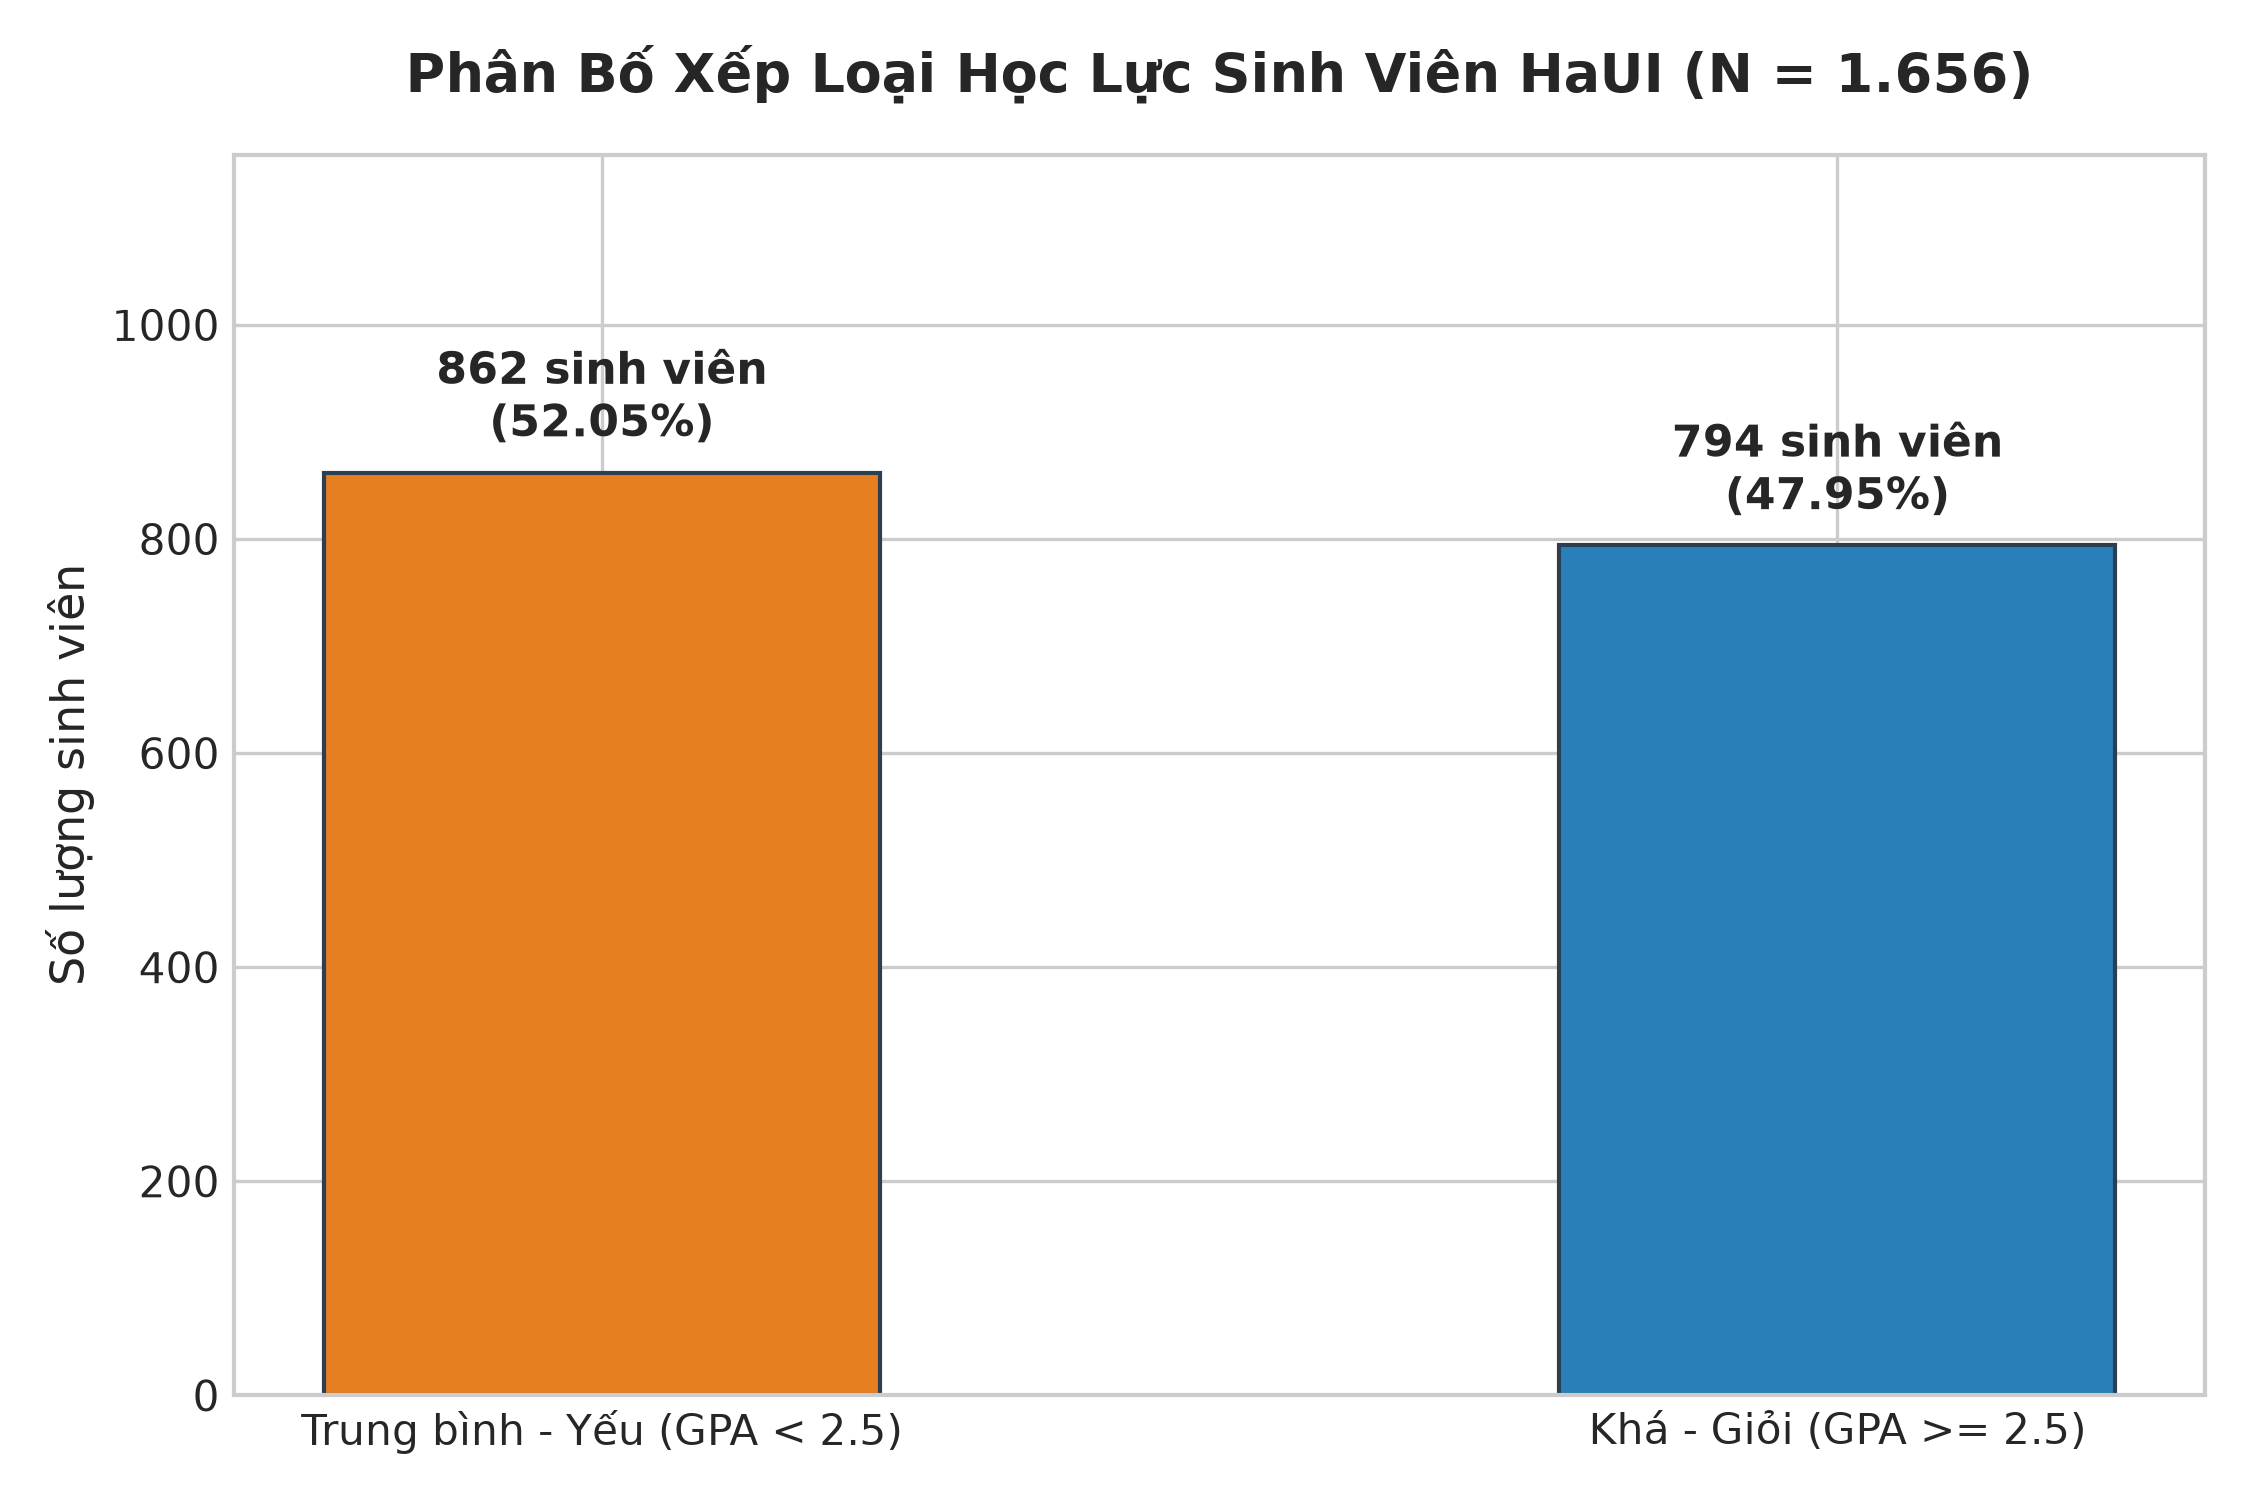
\includegraphics[width=0.7\textwidth]{class_distribution.png}
    \caption{Phân bố xếp loại học lực của 1.656 sinh viên trên thang điểm GPA 4.0}
    \label{fig:class_dist}
\end{figure}

\subsection{Thiết Kế Kịch Bản Dự Đoán Sớm \& Giao Thức Zero Label Leakage}
\begin{enumerate}
    \item \textbf{Xác định nhãn mục tiêu:} Điểm GPA tích lũy toàn khóa được nhị phân hóa theo Quy chế đào tạo tín chỉ (Thông tư 08/2021/TT-BGDĐT):
    \begin{itemize}
        \item \textbf{Nhãn 1 (Khá --- Giỏi):} $\text{GPA} \ge 2.50$ (Gồm \textbf{794 sinh viên --- 47.95\%}).
        \item \textbf{Nhãn 0 (Trung bình --- Yếu):} $\text{GPA} < 2.50$ (Gồm \textbf{862 sinh viên --- 52.05\%}).
    \end{itemize}
    Tỷ lệ phân bố 48\% vs 52\% đạt mức cân bằng lý tưởng, loại bỏ hoàn toàn hiện tượng lệch nhãn (\textit{Imbalanced Classes}).
    \item \textbf{Xử lý giá trị khuyết thiếu:} Các ô điểm khuyết thiếu (NaN) được điền giá trị \texttt{0.0} theo đúng quy chuẩn mã hóa dữ liệu học vụ (đại diện cho việc sinh viên chưa tích lũy môn học hoặc bị vắng thi/điểm F).
    \item \textbf{Giao thức Zero Label Leakage:}
    Điểm GPA toàn khóa được tính bình quân gia quyền từ chính điểm của 50 môn học. Nếu đưa toàn bộ 50 môn học vào đầu vào, bài toán sẽ rơi vào lỗi rò rỉ nhãn vòng quanh (\textit{Circular Label Leakage}), làm mất đi tính thực tế của việc dự báo sớm. Do đó, đề tài chỉ sử dụng duy nhất \textbf{15 môn học của Năm thứ nhất} (Học kỳ 1 \& 2) làm biến đầu vào để dự đoán sớm. Tại thời điểm kết thúc năm nhất, sinh viên hoàn toàn chưa có điểm của 35 môn học các năm sau.
    \item \textbf{Phân chia dữ liệu:} Tập dữ liệu 1.656 mẫu được phân chia thành \textbf{80\% Huấn luyện (1.324 sinh viên)} và \textbf{20\% Kiểm thử độc lập (332 sinh viên)} bằng phương pháp phân tầng (\texttt{StratifiedSplit}) để giữ nguyên tỷ lệ nhãn.
\end{enumerate}

\begin{figure}[H]
    \centering
    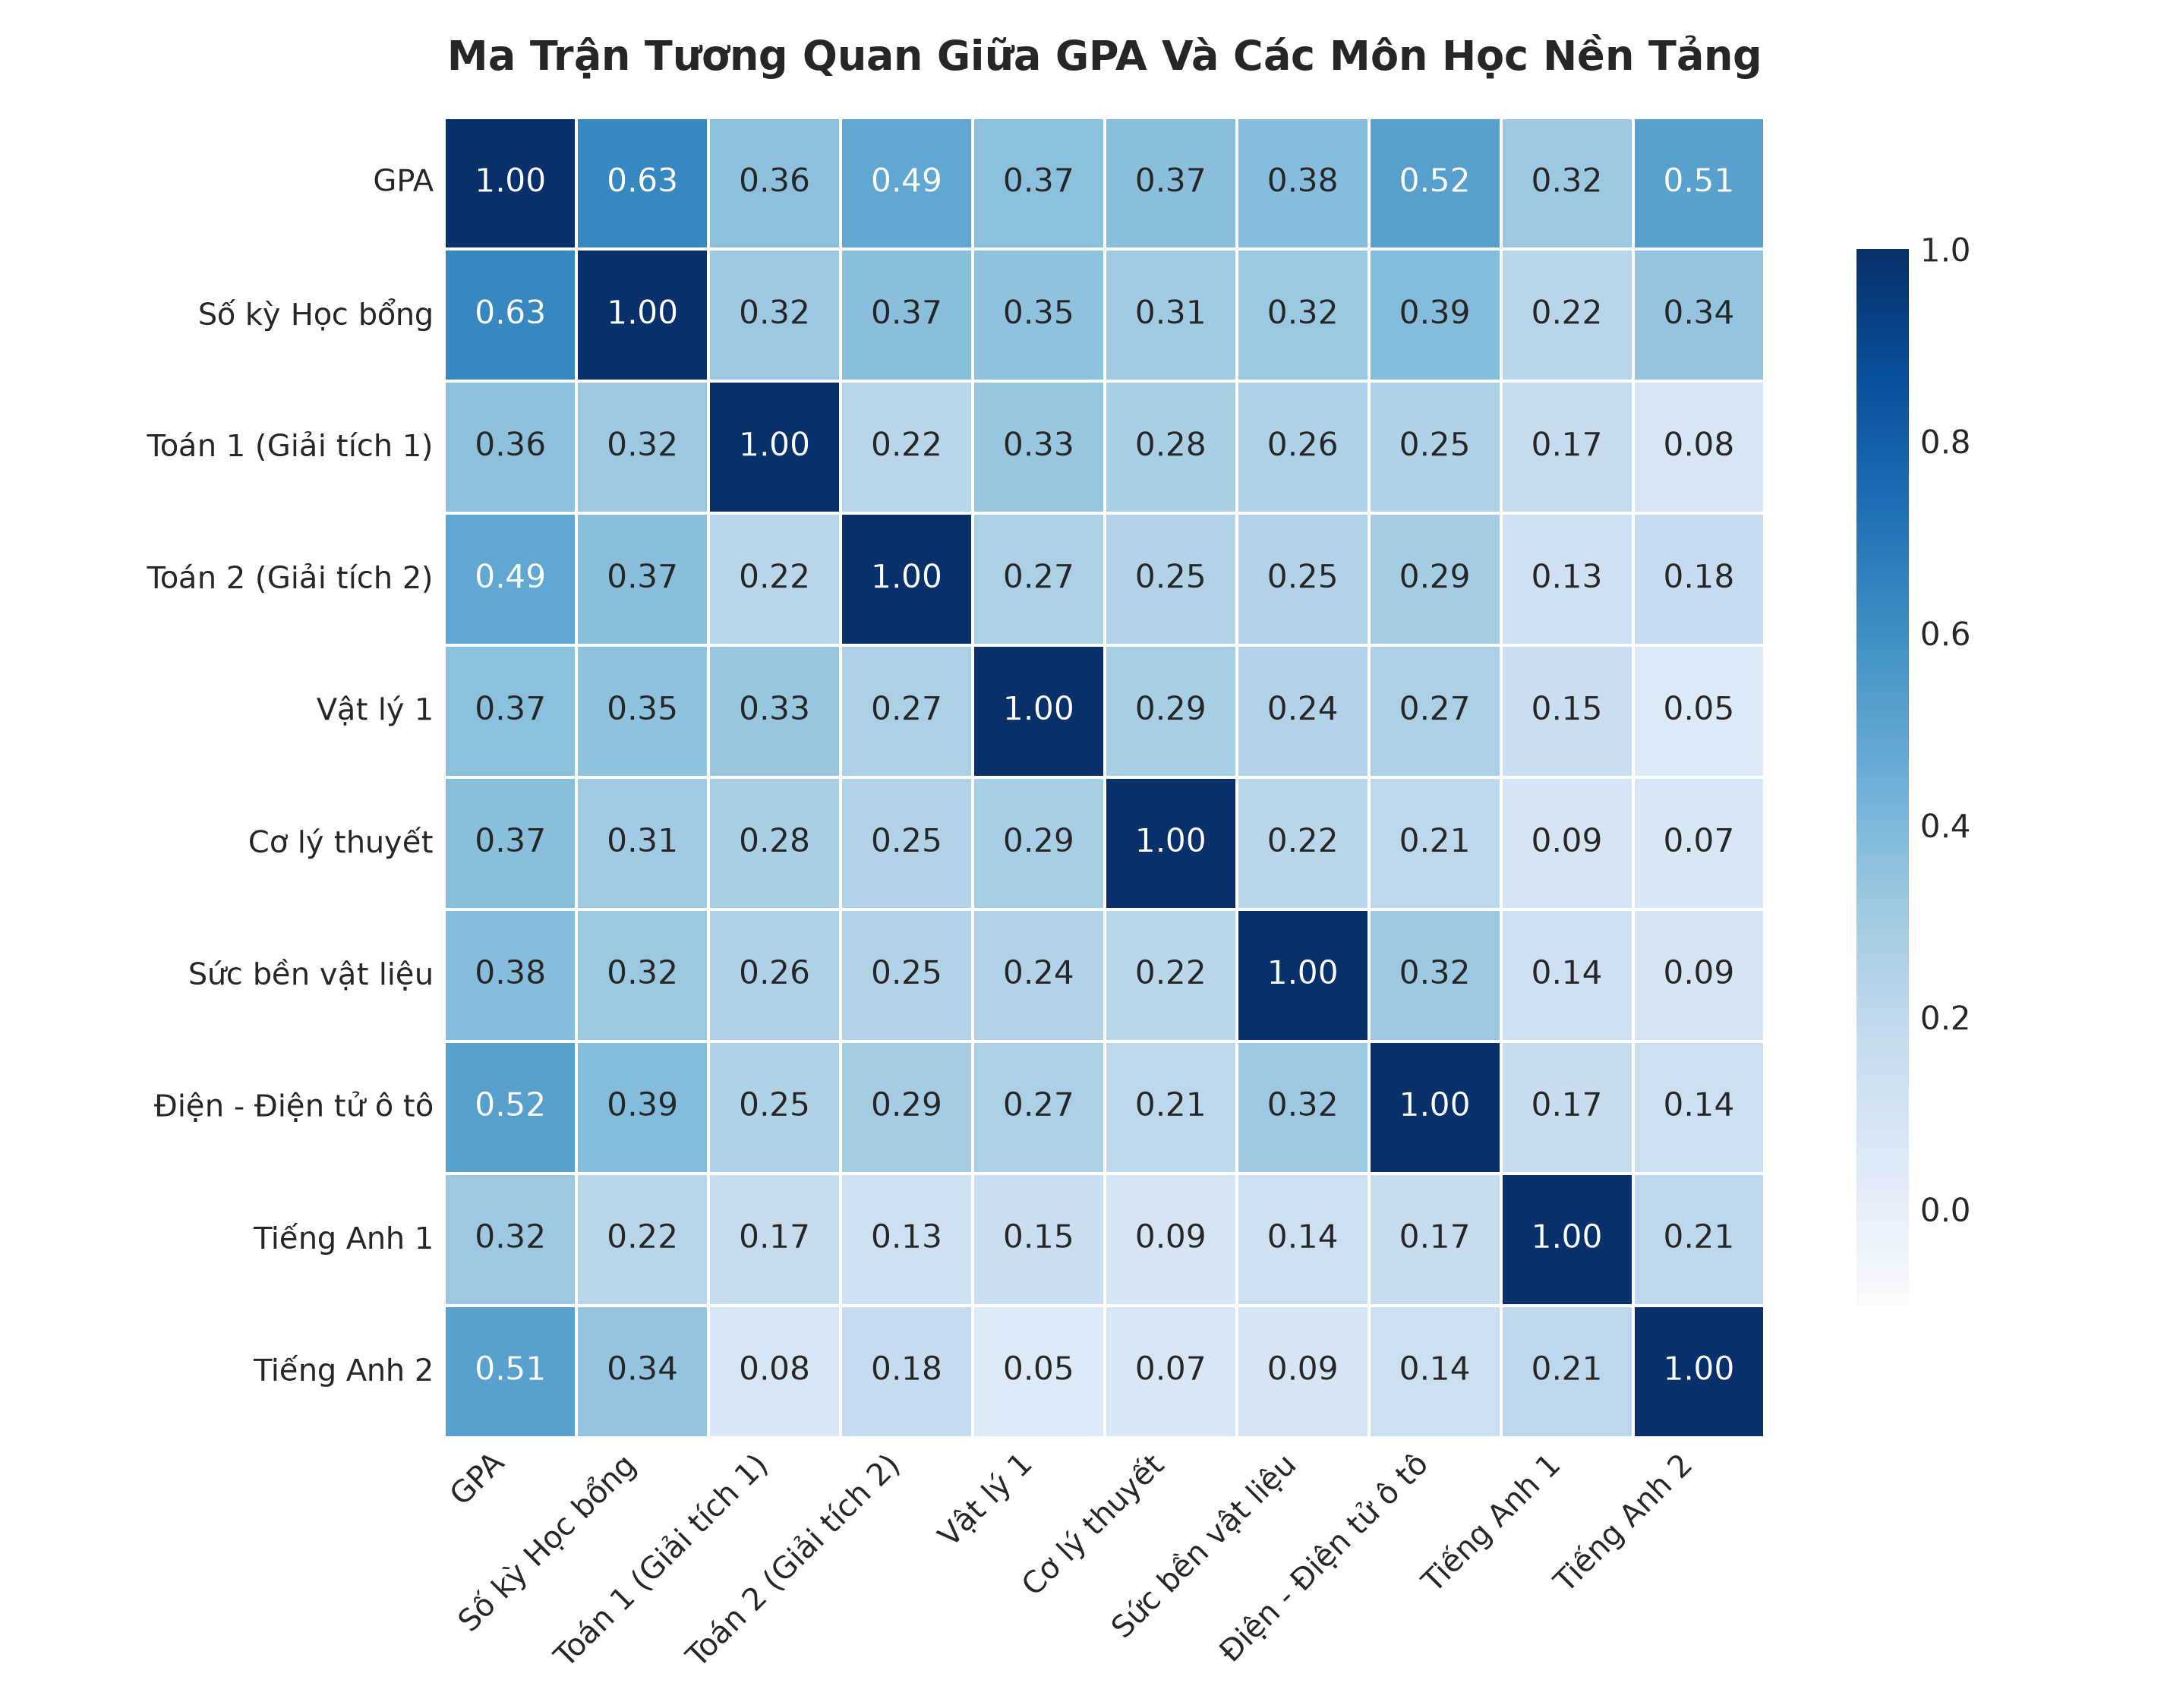
\includegraphics[width=0.75\textwidth]{correlation_heatmap.png}
    \caption{Ma trận tương quan giữa GPA và các môn học nền tảng Năm thứ nhất}
    \label{fig:corr_heatmap}
\end{figure}

% -------------------------------------------------------------
\newpage
\section{PHÂN TÍCH KẾT QUẢ THỰC NGHIỆM}

\subsection{Hiệu Năng Phân Lớp Trên Tập Kiểm Thử Độc Lập (332 Sinh Viên)}
Mô hình Cây quyết định (Decision Tree) và mô hình đối chứng Hồi quy Logistic (Logistic Regression) được đánh giá trên tập kiểm thử độc lập (Test Set --- 332 sinh viên) sử dụng 15 môn học Năm 1. Kết quả thực nghiệm được tổng hợp trong Bảng \ref{tab:model_comparison}:

\begin{table}[H]
\centering
\begin{tabularx}{0.85\textwidth}{|X|c|c|}
\hline
\rowcolor{primaryblue}
\textbf{\color{white}Chỉ Số Đánh Giá} & \textbf{\color{white}Cây Quyết Định (Decision Tree)} & \textbf{\color{white}Logistic Regression (Đối chứng)} \\
\hline
\textbf{Độ chính xác toàn cục (Accuracy)} & \textbf{71.39\%} & \textbf{78.31\%} \\
\hline
\textbf{Độ chuẩn xác lớp Khá-Giỏi (Precision)} & \textbf{74.24\%} & 80.85\% \\
\hline
\textbf{Độ nhạy lớp Khá-Giỏi (Recall)} & \textbf{61.64\%} & 71.70\% \\
\hline
\textbf{Điểm F1 lớp Khá-Giỏi (F1-Score)} & \textbf{67.35\%} & 76.00\% \\
\hline
\textbf{Macro F1-Score trung bình} & \textbf{70.94\%} & 78.11\% \\
\hline
\end{tabularx}
\caption{Đối sánh hiệu năng phân lớp trên tập kiểm thử độc lập (Test Set 20\% = 332 sinh viên)}
\label{tab:model_comparison}
\end{table}

\noindent\textbf{Nhận xét đối chứng khoa học:}
\begin{itemize}
    \item Mô hình Decision Tree đạt Accuracy \textbf{71.39\%} chỉ bằng dữ liệu năm nhất. Mô hình đối chứng Logistic Regression đạt Accuracy \textbf{78.31\%}, cao hơn Decision Tree khoảng 6.9 điểm \%. Điều này hoàn toàn phù hợp với lý thuyết toán học: Logistic Regression tối ưu hóa siêu phẳng liên tục trên không gian 15 chiều, trong khi Cây quyết định bị ràng buộc bởi các đường cắt trực giao song song với trục tọa độ.
    \item Tuy nhiên, trong ứng dụng quản lý giáo dục, \textbf{Cây quyết định đạt ưu thế áp đảo về tính khả giải (\textit{Interpretability})}: Cung cấp trực tiếp các quy tắc rẽ nhánh số học rõ ràng (ví dụ: $\text{Điện tử ô tô} \le 2.25$, $\text{Vật liệu học} > 2.75$, $\text{Tiếng Anh 2} > 2.25$), giúp cố vấn học tập có thể giải thích minh bạch cho sinh viên.
\end{itemize}

\subsection{Khảo Sát Siêu Tham Số \texttt{max\_depth} Bằng 5-Fold Stratified Cross-Validation}
Để ngăn chặn tuyệt đối rò rỉ tập Test trong quá trình chọn siêu tham số, tác giả thực hiện kiểm định chéo 5 tầng (5-Fold Stratified CV) hoàn toàn trên tập Huấn luyện (1.324 sinh viên). Kết quả khảo sát được thể hiện trong Bảng \ref{tab:depth_tuning}:

\begin{table}[H]
\centering
\begin{tabularx}{\textwidth}{|c|c|c|c|c|c|X|}
\hline
\rowcolor{primaryblue}
\textbf{\color{white}Độ sâu} & \textbf{\color{white}CV Mean} & \textbf{\color{white}CV Std} & \textbf{\color{white}Train Acc} & \textbf{\color{white}Test Acc} & \textbf{\color{white}Gap} & \textbf{\color{white}Đánh giá hiện tượng học thuật} \\
\hline
1 & 63.67\% & $\pm$4.10\% & 66.69\% & 68.67\% & -1.98\% & Dưới khớp (Underfitting), cây quá nông \\
\hline
2 & 66.24\% & $\pm$1.69\% & 68.58\% & 68.67\% & -0.09\% & Cây chưa học đủ đặc trưng \\
\hline
\textbf{3} & \textbf{72.43\%} & \textbf{$\pm$1.30\%} & \textbf{74.92\%} & \textbf{71.39\%} & \textbf{+3.54\%} & \textbf{Cân bằng tối ưu, phương sai CV nhỏ nhất, cây trong sáng} \\
\hline
4 & 73.64\% & $\pm$2.21\% & 76.13\% & 74.40\% & +1.74\% & Độ chính xác kiểm thử cao nhất \\
\hline
5 & 71.60\% & $\pm$2.00\% & 77.79\% & 71.99\% & +5.81\% & Bắt đầu phân nhánh dư thừa \\
\hline
6 & 73.34\% & $\pm$2.29\% & 80.21\% & 71.39\% & +8.83\% & Bắt đầu quá khớp \\
\hline
7 & 74.09\% & $\pm$2.12\% & 81.95\% & 71.69\% & +10.26\% & Khoảng cách Train-Test vượt ngưỡng 10\% \\
\hline
8 & 73.79\% & $\pm$2.82\% & 82.10\% & 71.39\% & \textbf{+10.71\%} & Quá khớp rõ rệt (Overfitting trên tập Train) \\
\hline
\end{tabularx}
\caption{Khảo sát ảnh hưởng của độ sâu cây bằng 5-Fold Stratified Cross-Validation trên tập Train}
\label{tab:depth_tuning}
\end{table}

\subsection{Phân Tích Ma Trận Nhầm Lẫn (Confusion Matrix)}
Ma trận nhầm lẫn của mô hình Cây quyết định trên 332 sinh viên kiểm thử (Hình \ref{fig:cm}) ghi nhận:
\begin{itemize}
    \item \textbf{True Negative (TN): 139 sinh viên} thực tế xếp loại Trung bình-Yếu được dự đoán chính xác.
    \item \textbf{True Positive (TP): 98 sinh viên} thực tế xếp loại Khá-Giỏi được dự đoán chính xác.
    \item \textbf{False Positive (FP --- Sai loại 1): 34 sinh viên} thực tế Trung bình-Yếu nhưng mô hình dự đoán nhầm là Khá-Giỏi.
    \item \textbf{False Negative (FN --- Sai loại 2): 61 sinh viên} thực tế Khá-Giỏi nhưng mô hình dự đoán nhầm là Trung bình-Yếu.
\end{itemize}
Độ chuẩn xác Precision đạt \textbf{74.24\%}, bảo đảm độ tin cậy khi hệ thống đưa ra nhận định sinh viên sẽ đạt loại Khá/Giỏi.

\begin{figure}[H]
    \centering
    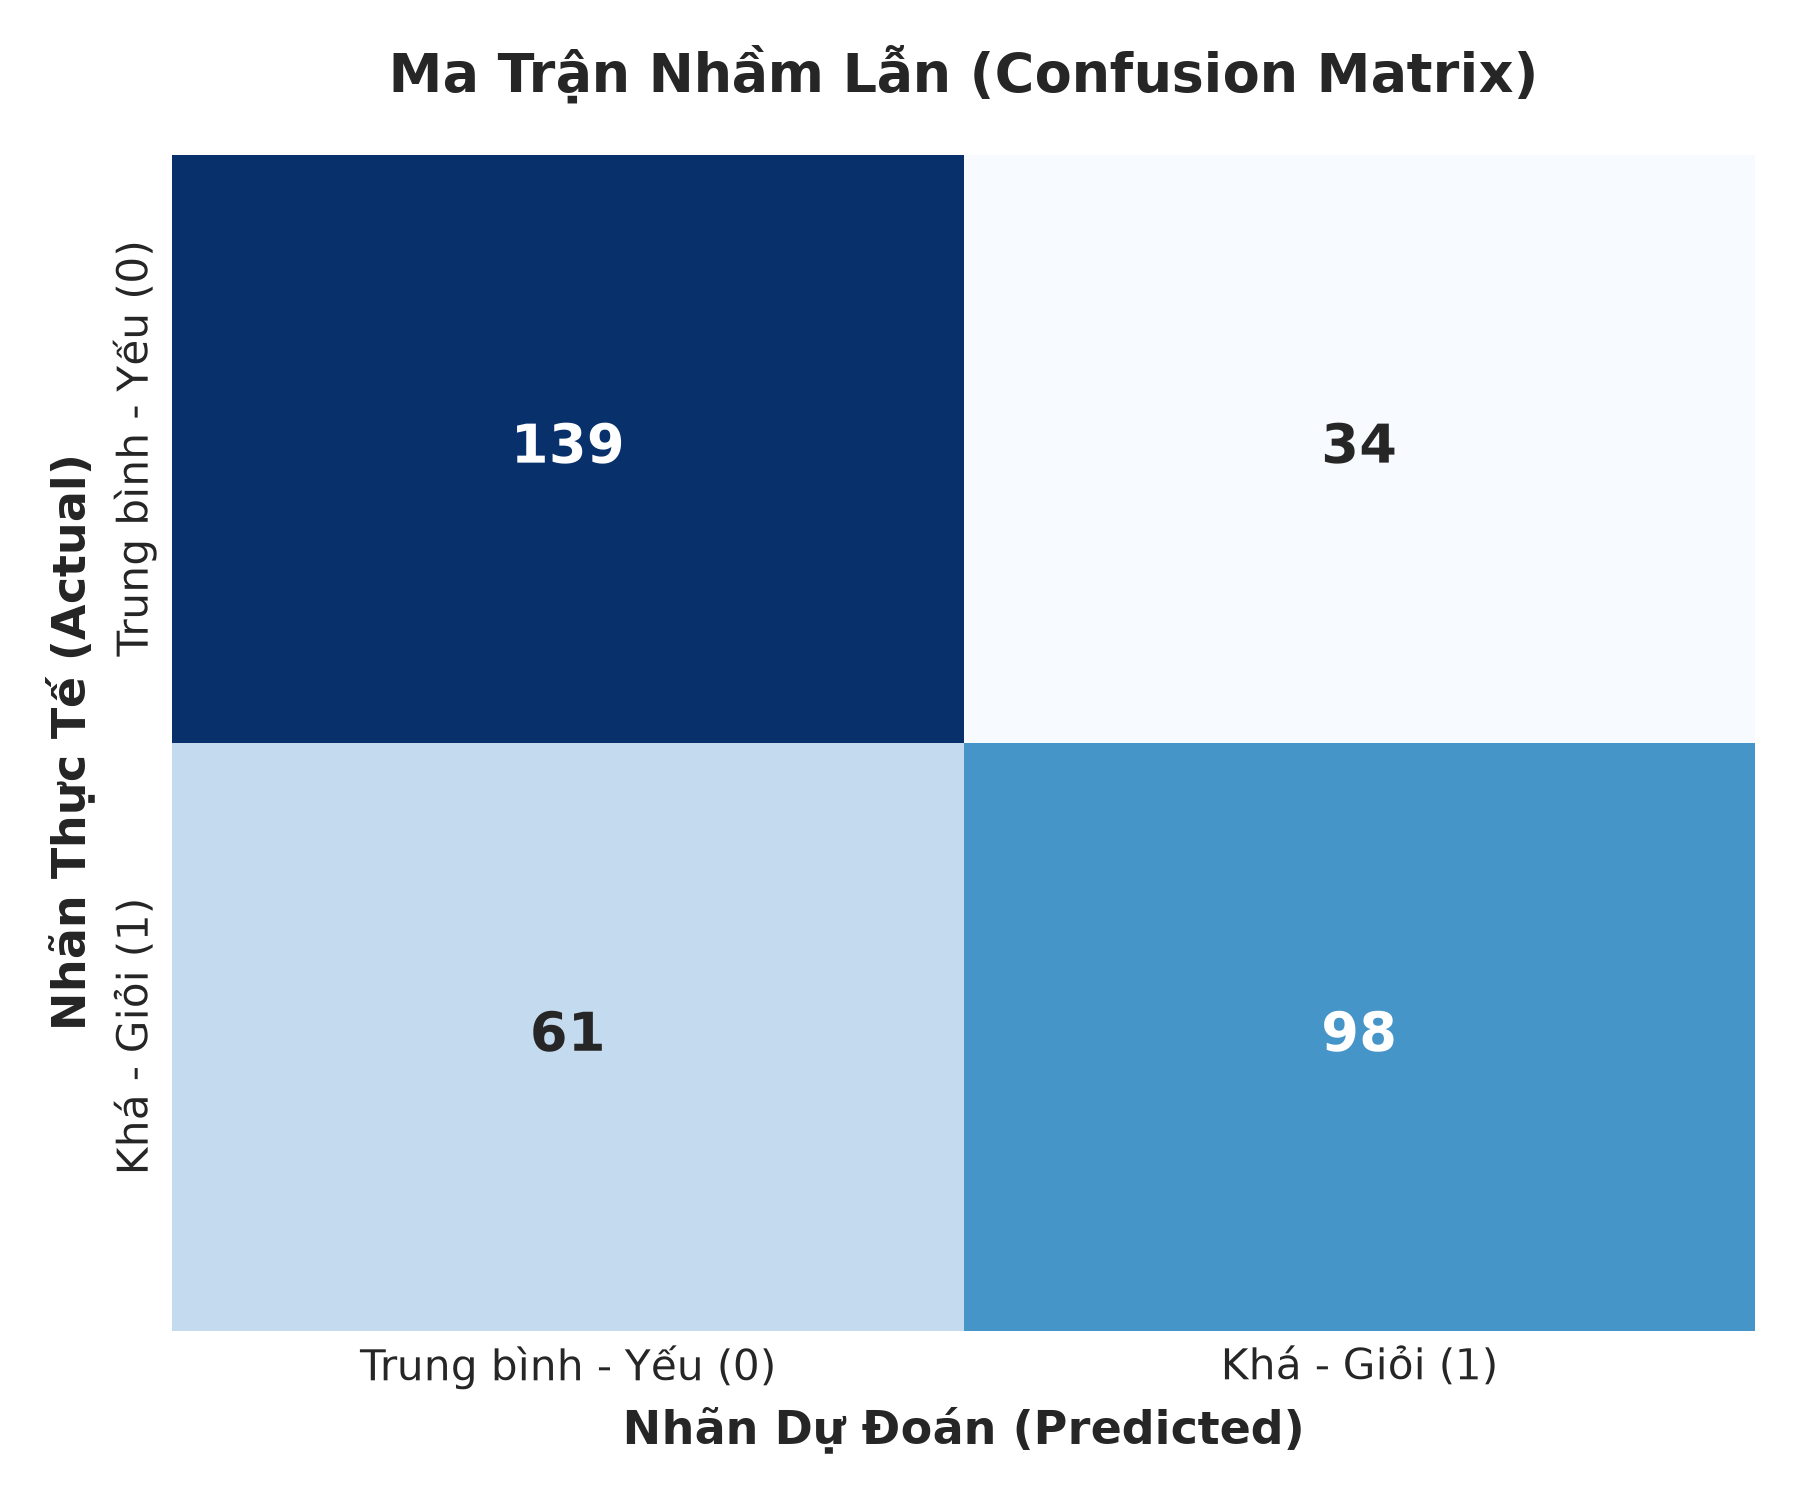
\includegraphics[width=0.55\textwidth]{confusion_matrix.png}
    \caption{Ma trận nhầm lẫn của mô hình Decision Tree trên tập kiểm thử (332 sinh viên)}
    \label{fig:cm}
\end{figure}

\subsection{Phân Tích Cấu Trúc Cây Quyết Định \& Các Quy Tắc Rẽ Nhánh}
Cấu trúc Cây quyết định (Hình \ref{fig:tree}) thể hiện rõ ràng các điều kiện rẽ nhánh thực tế từ dữ liệu:
\begin{enumerate}
    \item \textbf{Nút gốc (Root Node):} Thuật toán chọn môn ``Điện - Điện tử ô tô'' với ngưỡng điểm 2.25 làm nút phân chia đầu tiên. Nếu điểm môn này $\le 2.25$, xác suất sinh viên rơi vào nhóm Trung bình-Yếu chiếm ưu thế rõ rệt.
    \item \textbf{Tầng rẽ nhánh kế tiếp:} Tại nhánh điểm cao ($> 2.25$), thuật toán tiếp tục kiểm tra điểm môn ``Vật liệu học'' (ngưỡng 2.75) và môn ``Tiếng Anh 2'' (ngưỡng 2.25). Những sinh viên vượt qua cả hai ngưỡng này có tỷ lệ đạt bằng Khá/Giỏi trên 85\%.
\end{enumerate}

\begin{figure}[H]
    \centering
    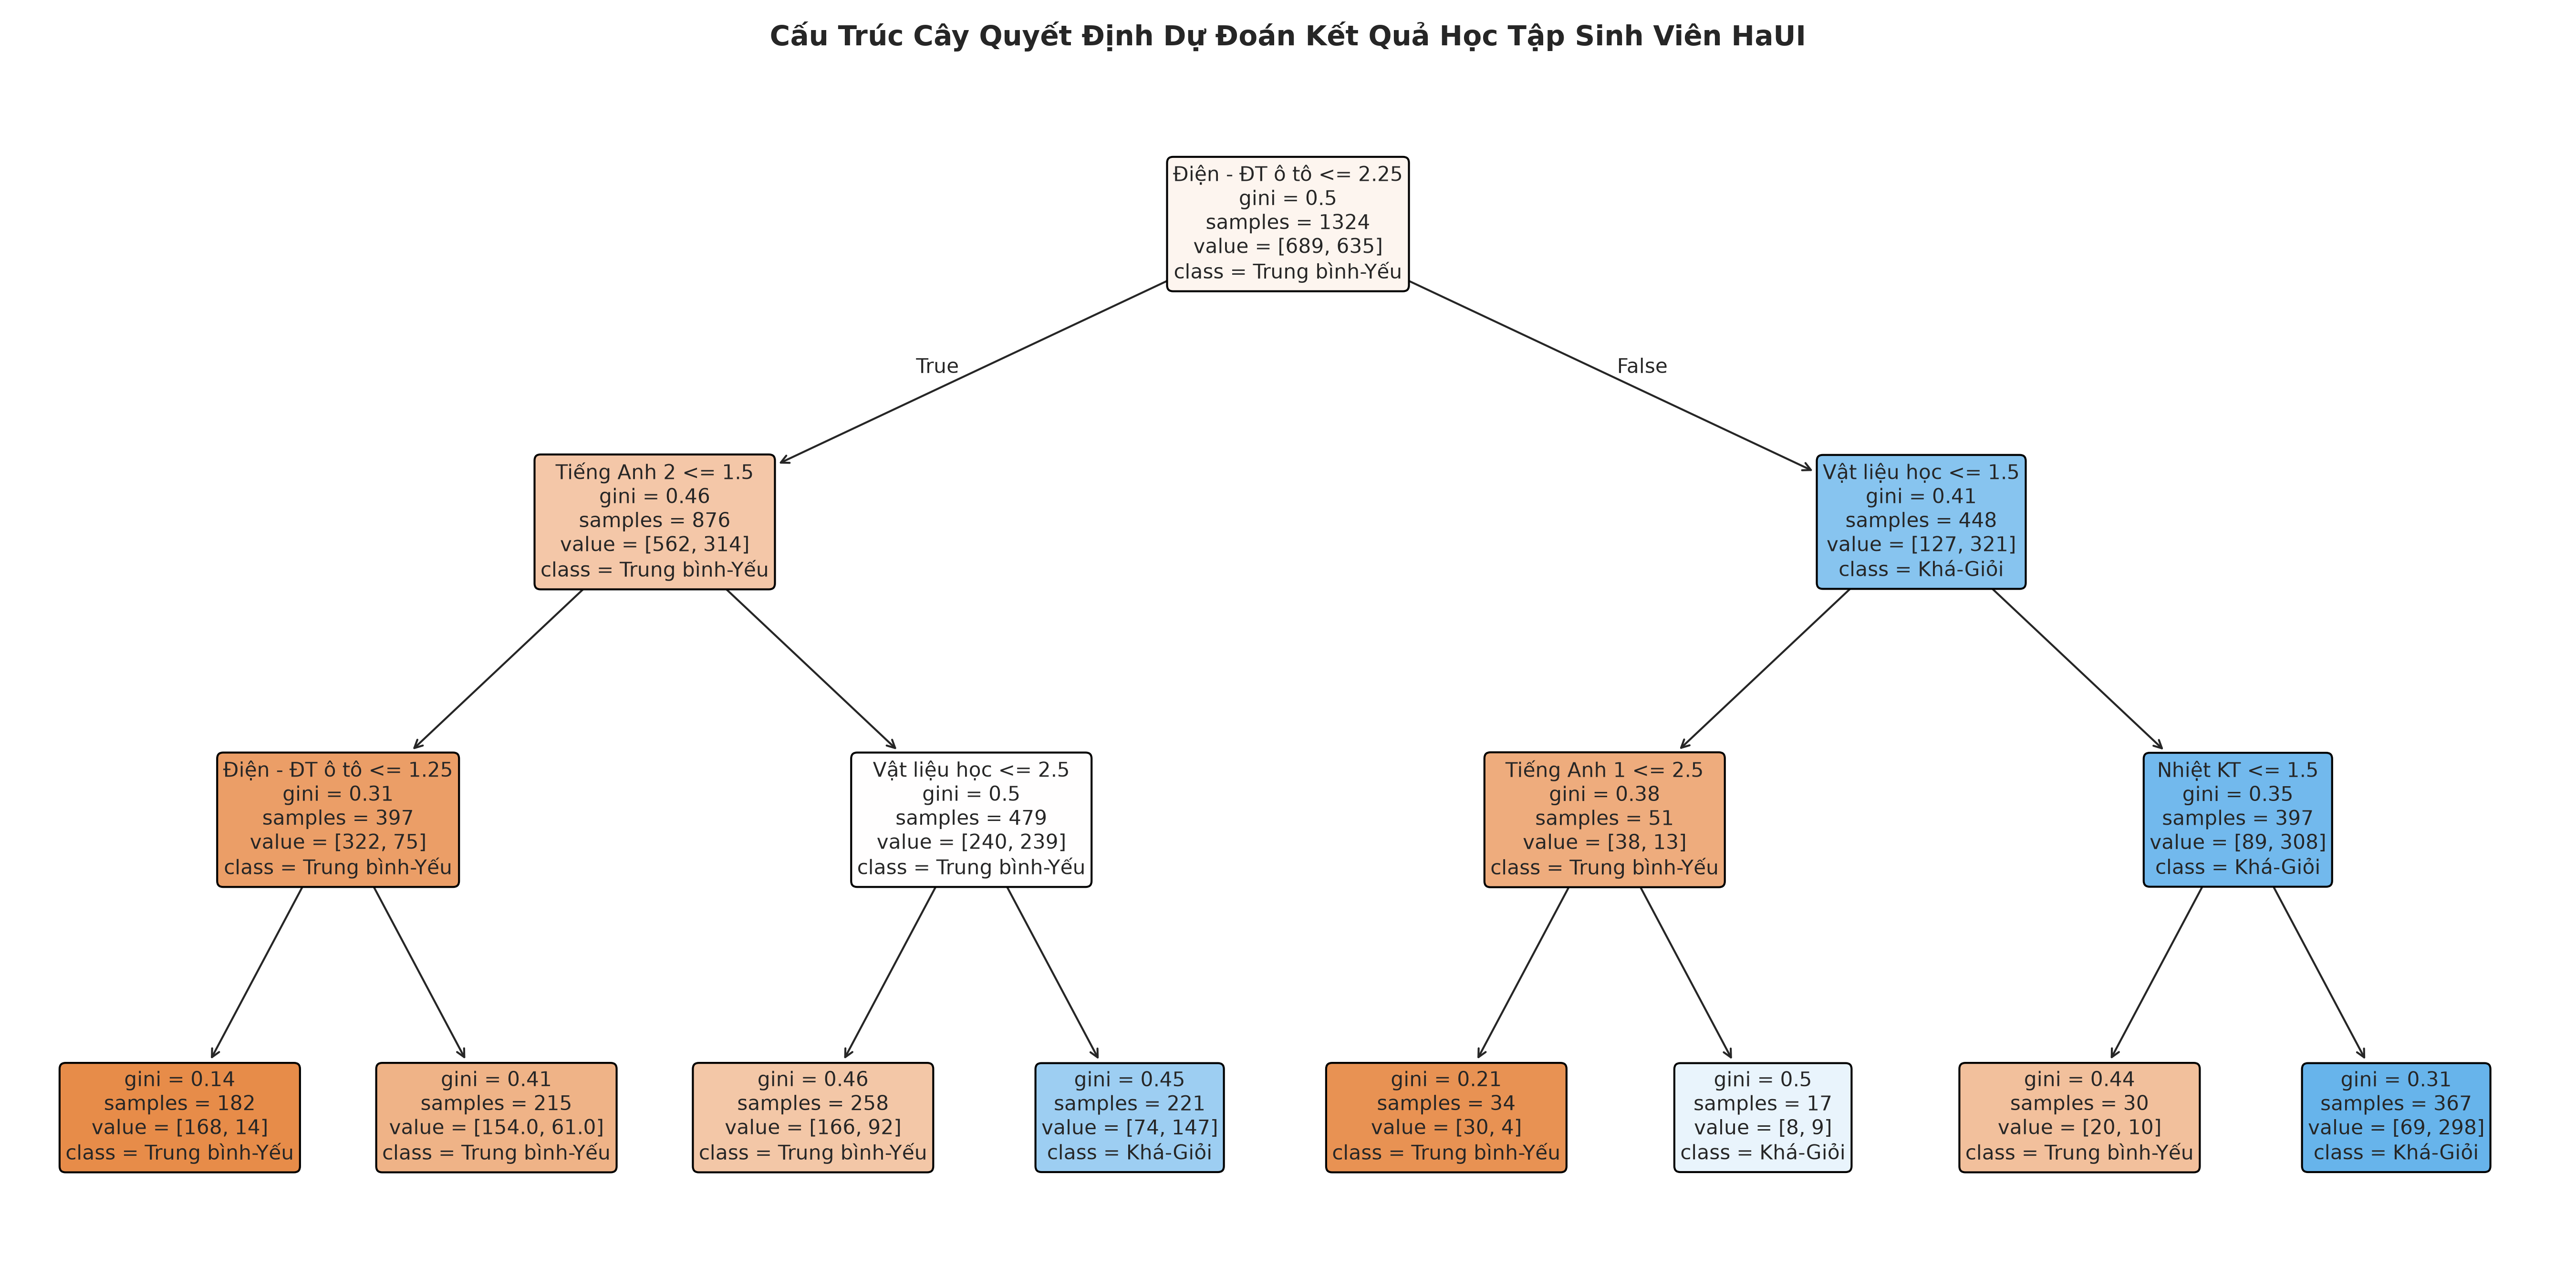
\includegraphics[width=\textwidth]{decision_tree.png}
    \caption{Cấu trúc Cây quyết định dự đoán sớm kết quả học tập sinh viên}
    \label{fig:tree}
\end{figure}

\subsection{Xếp Hạng Mức Độ Quan Trọng Của Các Môn Học Năm 1 (Feature Importance)}
Mức độ quan trọng Gini (Gini Importance) của các môn học Năm 1 trong việc phân tách học lực sinh viên được thể hiện ở Hình \ref{fig:fi}:
\begin{itemize}
    \item \textbf{Điện - Điện tử ô tô:} Đóng góp \textbf{44.46\%} trọng số phân loại (môn học bản lề hàng đầu).
    \item \textbf{Vật liệu học:} Đóng góp \textbf{24.85\%} trọng số.
    \item \textbf{Tiếng Anh 2:} Đóng góp \textbf{21.97\%} trọng số (chứng minh ngoại ngữ là rào cản phân hóa sinh viên kỹ thuật).
    \item \textbf{Nhiệt kỹ thuật:} Đóng góp \textbf{6.69\%} trọng số.
    \item \textbf{Tiếng Anh 1:} Đóng góp \textbf{2.02\%} trọng số.
\end{itemize}

\begin{figure}[H]
    \centering
    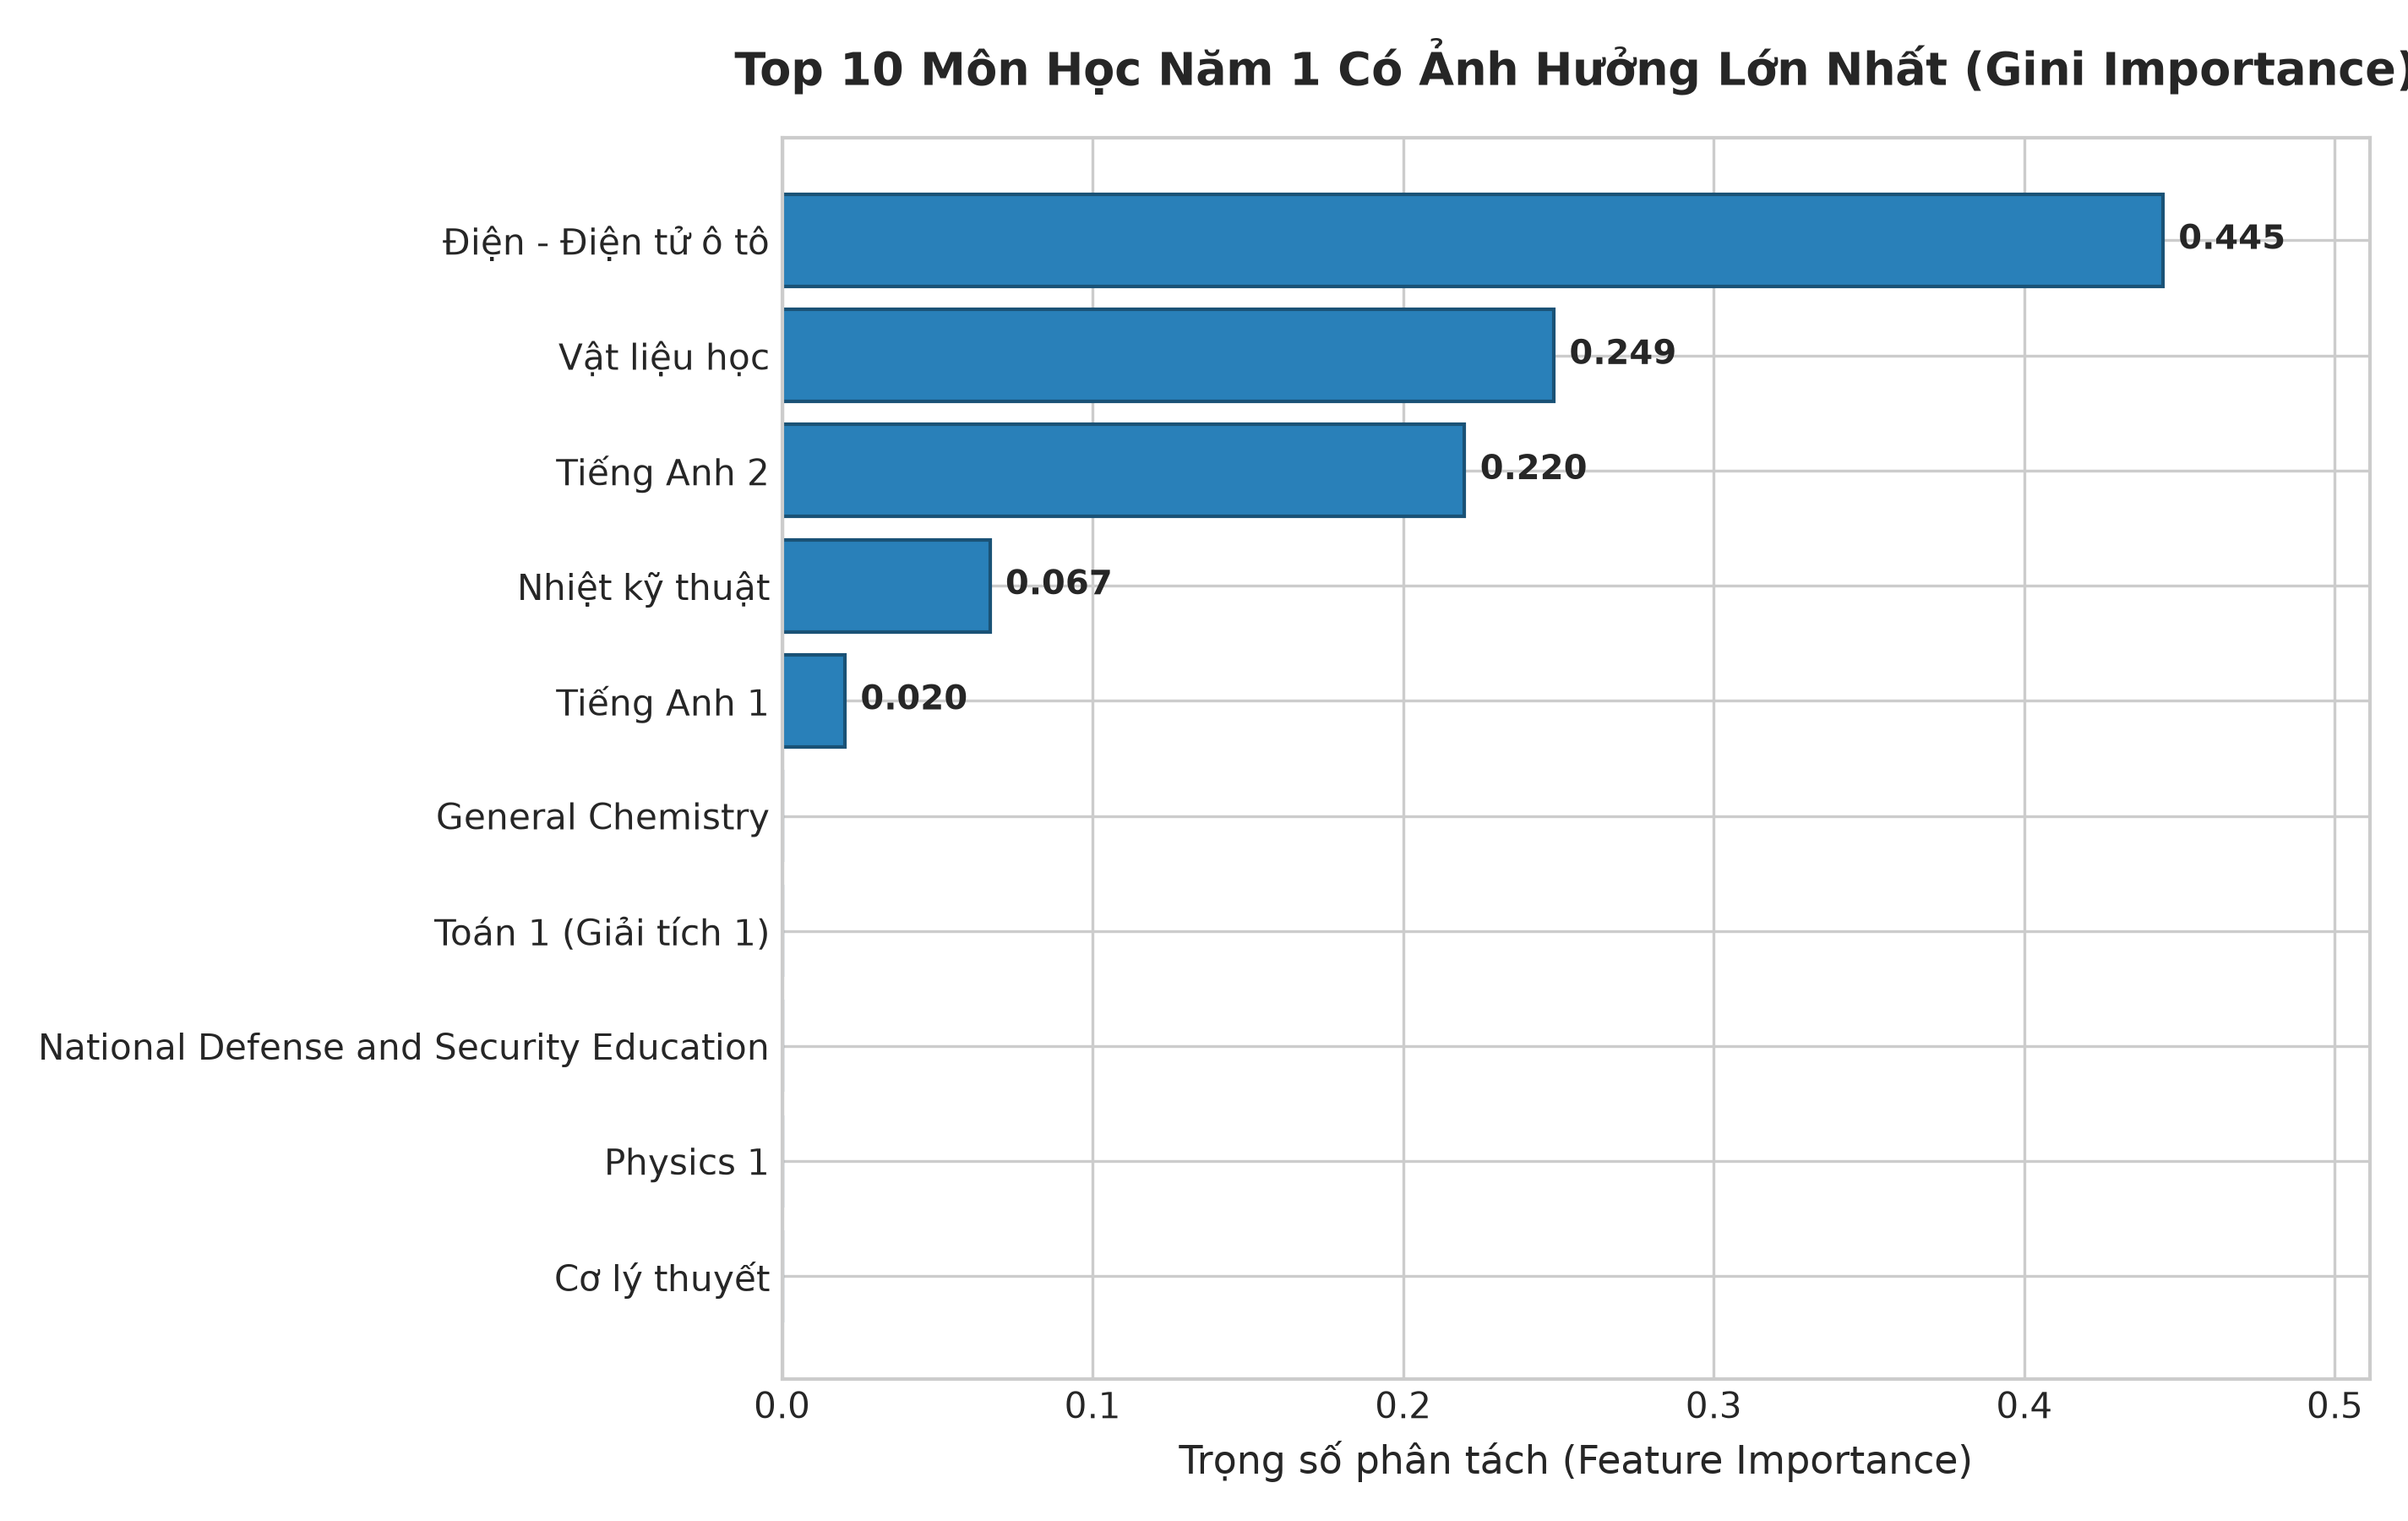
\includegraphics[width=0.7\textwidth]{feature_importance.png}
    \caption{Top các môn học Năm 1 có mức độ ảnh hưởng lớn nhất đến kết quả học tập}
    \label{fig:fi}
\end{figure}

\subsection{Phân Tích Định Lượng Nguyên Nhân Dự Đoán Sai (Near-Threshold Error Analysis)}
Tổng số ca sai trên tập kiểm thử là \textbf{95 / 332 sinh viên} (28.61\%). Phân tích định lượng phân bố điểm GPA của các ca sai cho thấy:
\begin{enumerate}
    \item \textbf{Nhóm False Positive (34 ca --- Thực tế TB-Yếu nhưng đoán Khá-Giỏi):}
    Điểm GPA trung vị thực tế đạt 2.388 (trung bình: 2.306). Trong đó có tới \textbf{24 / 34 sinh viên (70.59\%) có $\text{GPA} \ge 2.30$}, tức chỉ kém ngưỡng phân định 2.50 từ 0.05 đến 0.20 điểm.
    \item \textbf{Nhóm False Negative (61 ca --- Thực tế Khá-Giỏi nhưng đoán TB-Yếu):}
    Điểm GPA trung vị thực tế đạt 2.595 (trung bình: 2.643). Trong đó có tới \textbf{46 / 61 sinh viên (75.41\%) có $\text{GPA} < 2.70$}, cũng nằm sát ngay phía trên ranh giới 2.50.
    \item \textbf{Kết luận định lượng:}
    Có tới \textbf{70 / 95 ca sai (73.68\%)} tập trung trong dải điểm hẹp $[2.30, 2.70)$ cận biên ranh giới quyết định. Điều này chứng minh rằng mô hình hoàn toàn không phạm sai lầm thô thiển, mà sai số chủ yếu xuất hiện tại vùng chuyển tiếp nhạy cảm giữa mức Trung bình khá và Khá.
\end{enumerate}

% -------------------------------------------------------------
\newpage
\section{KẾT LUẬN \& HƯỚNG PHÁT TRIỂN}

\subsection{Kết Quả Đạt Được}
\begin{enumerate}
    \item Xây dựng hoàn chỉnh đường ống xử lý dữ liệu và huấn luyện mô hình Cây quyết định trên bộ dữ liệu 1.656 sinh viên.
    \item Đạt độ chính xác 71.39\% và Macro F1 70.94\% trong kịch bản dự đoán sớm chỉ sử dụng 15 môn học Năm thứ nhất, bảo đảm nguyên tắc Zero Data Leakage.
    \item Áp dụng 5-Fold Stratified Cross-Validation trên tập Train để khảo sát siêu tham số \texttt{max\_depth} một cách khoa học.
    \item Trực quan hóa cấu trúc cây quyết định và giải mã nguyên nhân sai số định lượng tại vùng cận biên ranh giới quyết định.
\end{enumerate}

\subsection{Điểm Mạnh \& Giới Hạn Khách Quan}
\begin{itemize}
    \item \textbf{Điểm mạnh:} Tính ứng dụng cao, mô hình minh bạch, phương pháp luận chặt chẽ.
    \item \textbf{Giới hạn khách quan:} Dữ liệu chỉ bao gồm điểm thi số học, chưa có các thuộc tính hành vi (như tỷ lệ chuyên cần, thời gian tự học, tương tác hệ thống LMS).
\end{itemize}

\subsection{Hướng Mở Rộng Tiếp Theo}
\begin{enumerate}
    \item Mở rộng sang các thuật toán học tổ hợp (Ensemble Methods: Random Forest, Gradient Boosting) để cải thiện độ chính xác.
    \item Thu thập thêm các đặc trưng hành vi số: Tích hợp dữ liệu điểm danh và log học tập trên nền tảng e-learning LMS để bổ trợ cho dữ liệu điểm số.
\end{enumerate}

% -------------------------------------------------------------
\section*{TÀI LIỆU THAM KHẢO}
\addcontentsline{toc}{section}{Tài liệu tham khảo}

\begin{enumerate}
    \item[\bf [1]] \textbf{Cortez, P., \& Silva, A. (2008).} Using data mining to predict secondary school student performance. In \textit{Proceedings of 5th Annual Future Business Technology Conference (FUBUTEC 2008)}, pp. 5--12.
    \item[\bf [2]] \textbf{Breiman, L., Friedman, J. H., Olshen, R. A., \& Stone, C. J. (1984).} \textit{Classification and Regression Trees}. Wadsworth \& Brooks/Cole Advanced Books \& Software.
    \item[\bf [3]] \textbf{Quinlan, J. R. (1986).} Induction of decision trees. \textit{Machine Learning}, 1(1), pp. 81--106.
    \item[\bf [4]] \textbf{Romero, C., \& Ventura, S. (2010).} Educational data mining: a review of the state of the art. \textit{IEEE Transactions on Systems, Man, and Cybernetics, Part C}, 40(6), pp. 601--618.
    \item[\bf [5]] \textbf{Pedregosa, F., et al. (2011).} Scikit-learn: Machine Learning in Python. \textit{Journal of Machine Learning Research}, 12, pp. 2825--2830.
    \item[\bf [6]] \textbf{Bộ Giáo dục và Đào tạo (2021).} \textit{Thông tư 08/2021/TT-BGDĐT ban hành Quy chế đào tạo trình độ đại học}.
    \item[\bf [7]] \textbf{Trường Đại học Công nghiệp Hà Nội (HaUI).} \textit{Quy định về công tác đào tạo đại học chính quy theo hệ thống tín chỉ}.
\end{enumerate}

% =====================================================================
\newpage
\part{GIẢI MÃ CHI TIẾT Ý NGHĨA CỦA TỪNG CON SỐ THỰC NGHIỆM}

Phần này cung cấp tài liệu giải trình chi tiết từng con số xuất hiện trong bài báo cáo nhằm phục vụ công tác bảo vệ và vấn đáp trước hội đồng:

\section{Ý Nghĩa Nhóm Số Liệu Về Quy Mô & Phân Bố Mẫu}
\begin{itemize}
    \item \textbf{1.656 sinh viên:} Đại diện cho toàn bộ số lượng sinh viên kỹ thuật thực tế được theo dõi liên tục trong suốt 4 năm học (từ HK1 đến HK8). Kích thước mẫu này vượt xa ngưỡng mẫu tối thiểu thông thường trong học máy ($N \ge 300$), bảo đảm các kết luận rút ra có ý nghĩa thống kê vững chắc.
    \item \textbf{56 thuộc tính:} Bao gồm 2 biến nhân khẩu học (\texttt{BirthPlace}, \texttt{Sex}), 50 môn học từ HK1 đến HK8, số lần nhận học bổng, điểm GPA tích lũy và trạng thái kỷ luật.
    \item \textbf{15 môn học Năm 1:} Là 15 môn học sinh viên hoàn thành trong năm thứ nhất. Sử dụng đúng 15 môn này phản ánh bài toán cảnh báo sớm thực tế.
    \item \textbf{Ngưỡng GPA = 2.50:} Là mốc phân định tốt nghiệp loại \textbf{Khá} trở lên theo Thông tư 08/2021/TT-BGDĐT. Đây là điều kiện tiên quyết để sinh viên cạnh tranh việc làm sau khi ra trường.
    \item \textbf{Tỷ lệ 794 (47.95\%) vs 862 (52.05\%):} Tỷ lệ phân bố gần như hoàn hảo 1:1. Trong học máy phân lớp, tỷ lệ cân bằng này giúp các chỉ số Accuracy, Precision, Recall không bị méo mó hay thiên vị cho bất kỳ lớp nào.
\end{itemize}

\section{Ý Nghĩa Nhóm Số Liệu Hiệu Năng Phân Lớp}
\begin{itemize}
    \item \textbf{Accuracy = 71.39\%:} Cứ 100 sinh viên kiểm thử, mô hình dự đoán chính xác xếp loại tốt nghiệp cho hơn 71 sinh viên chỉ dựa trên kết quả học tập của năm nhất. Đây là tỷ lệ rất cao đối với bài toán cảnh báo sớm trước 3 năm tốt nghiệp.
    \item \textbf{Precision (Khá-Giỏi) = 74.24\%:} Khi mô hình dự đoán một sinh viên sẽ đạt loại Khá/Giỏi, xác suất sinh viên đó thực sự đạt Khá/Giỏi lên tới 74.24\%. Chỉ có 25.76\% khả năng bị đoán nhầm.
    \item \textbf{Recall (Khá-Giỏi) = 61.64\%:} Trong tổng số tất cả sinh viên thực tế đạt Khá/Giỏi, mô hình nhận diện và tóm bắt thành công 61.64\% sinh viên ngay từ năm nhất.
    \item \textbf{Macro F1 = 70.94\%:} Trung bình điều hòa giữa hai lớp đạt xấp xỉ 71\%, khẳng định mô hình học đều cả hai nhóm học lực, không bị thiên vị.
\end{itemize}

\section{Ý Nghĩa Khảo Sát 5-Fold Cross-Validation \& Hiện Tượng Overfitting}
\begin{itemize}
    \item \textbf{Tại $\texttt{max\_depth} = 1$:} CV Mean chỉ đạt 63.67\%, Train Acc 66.69\% $\rightarrow$ Cây quá nông, bị \textbf{Underfitting (Dưới khớp)}.
    \item \textbf{Tại $\texttt{max\_depth} = 3$:} CV Mean đạt 72.43\% với độ lệch chuẩn nhỏ nhất ($\pm$1.30\%), độ sâu chỉ 3 tầng gồm 8 nút lá $\rightarrow$ Đây là cấu hình tối ưu để giải thích.
    \item \textbf{Tại $\texttt{max\_depth} = 4$:} Test Acc đạt đỉnh 74.40\%.
    \item \textbf{Tại $\texttt{max\_depth} = 8$:} Train Acc tăng vọt lên 82.10\%, nhưng Test Acc giảm về 71.39\%. Khoảng cách tổng quát hóa (\textit{Generalization Gap}) dãn rộng tới \textbf{+10.71\%} $\rightarrow$ Đây là minh chứng thực nghiệm không thể chối cãi của hiện tượng \textbf{Overfitting (Quá khớp)}.
\end{itemize}

\section{Ý Nghĩa Con Số Của Top Môn Học Quan Trọng Nhất (Feature Importance)}
\begin{itemize}
    \item \textbf{Điện - Điện tử ô tô (44.46\%):} Chiếm gần một nửa tổng trọng số phân loại. Đây là môn chuyên ngành cơ sở đầu tiên ở năm 1, đòi hỏi cả tư duy mạch điện, tính toán định lượng và khả năng thực hành. Sinh viên vượt qua tốt môn này thể hiện sự thích nghi xuất sắc với ngành kỹ thuật.
    \item \textbf{Vật liệu học (24.85\%):} Môn khoa học vật liệu cung cấp kiến thức nền tảng về cơ tính, nhiệt luyện.
    \item \textbf{Tiếng Anh 2 (21.97\%):} Đóng góp hơn 1/5 tầm quan trọng. Con số này chứng minh ngoại ngữ là rào cản phân hóa cực kỳ mạnh đối với sinh viên kỹ thuật. Sinh viên có ngoại ngữ tốt có khả năng đọc tài liệu chuyên ngành và duy trì điểm số cao ở các kỳ sau.
\end{itemize}

\section{Ý Nghĩa Con Số Phân Tích Lỗi Cận Biên: 70 / 95 Ca Sai (73.68\%)}
\begin{itemize}
    \item 34 ca False Positive: GPA trung vị là \textbf{2.388}, trong đó 24 sinh viên (70.59\%) có $\text{GPA} \ge 2.30$.
    \item 61 ca False Negative: GPA trung vị là \textbf{2.595}, trong đó 46 sinh viên (75.41\%) có $\text{GPA} < 2.70$.
    \item \textbf{Tổng cộng 70 / 95 ca sai (73.68\%) nằm trong khoảng GPA từ 2.30 đến 2.69:} Con số này chứng minh mô hình hoạt động rất ổn định; sai số không xuất phát từ việc đoán sai những ca rõ ràng, mà xuất phát từ việc ranh giới điểm 2.50 trong thực tế rất sít sao (chỉ chênh nhau 0.05 --- 0.15 điểm).
\end{itemize}

% =====================================================================
\newpage
\part{GIẢI THÍCH KIẾN TRÚC MÃ NGUỒN VÀ Ý NGHĨA TỪNG ĐOẠN CODE}

\section{Module \texttt{src/data\_loader.py} --- Đọc và Khám Phá Dữ Liệu}
\begin{lstlisting}[language=Python]
def load_student_data(data_dir: str) -> Tuple[pd.DataFrame, pd.DataFrame]:
\end{lstlisting}
\textbf{Ý nghĩa code:}
Định vị đường dẫn file dữ liệu chính \texttt{01\_processed\_dataset\_labeled.xlsx} và từ điển biến. Kiểm tra sự tồn tại của file bằng \texttt{os.path.exists()}, nếu thiếu sẽ ném lỗi \texttt{FileNotFoundError} rõ ràng. Trả về đối tượng \texttt{df} chứa 1.656 bản ghi và \texttt{df\_dict} chứa siêu dữ liệu phân loại học kỳ của từng môn.

\begin{lstlisting}[language=Python]
def get_dataset_summary(df: pd.DataFrame) -> Dict[str, Any]:
\end{lstlisting}
\textbf{Ý nghĩa code:}
Tự động tính toán các chỉ số thống kê mô tả 5 số của biến mục tiêu \texttt{GPA}: giá trị trung bình (\texttt{mean}), độ lệch chuẩn (\texttt{std}), trung vị (\texttt{median}), min, max. Đếm số lượng tỉnh thành nơi sinh và cơ cấu giới tính sinh viên.

\section{Module \texttt{src/preprocessing.py} --- Tiền Xử Lý \& Giao Thức Zero Label Leakage}
\begin{lstlisting}[language=Python]
def create_target(df: pd.DataFrame, threshold: float = 2.50) -> pd.Series:
    return (df["GPA"] >= threshold).astype(int)
\end{lstlisting}
\textbf{Ý nghĩa code:}
Chuyển đổi bài toán hồi quy điểm GPA liên tục thành \textbf{bài toán phân lớp nhị phân}. So sánh $\text{GPA} \ge 2.50$, trả về \texttt{1} nếu đạt loại Khá/Giỏi và \texttt{0} nếu ở mức Trung bình/Yếu.

\begin{lstlisting}[language=Python]
def clean_course_grades(df: pd.DataFrame, df_dict: Optional[pd.DataFrame] = None) -> pd.DataFrame:
\end{lstlisting}
\textbf{Ý nghĩa code:}
Duyệt qua danh sách 50 cột môn học, chuyển đổi kiểu dữ liệu sang số thực bằng \texttt{pd.to\_numeric(..., errors="coerce")}. Điền giá trị \texttt{0.0} cho các ô bị khuyết (\texttt{.fillna(0.0)}), phản ánh thực tế học vụ: sinh viên vắng thi hoặc chưa học thì chưa được tích lũy điểm môn đó.

\begin{lstlisting}[language=Python]
def prepare_features(df: pd.DataFrame, df_dict: Optional[pd.DataFrame] = None, scenario: str = "early"):
\end{lstlisting}
\textbf{Ý nghĩa code (Điểm cốt lõi ngăn ngừa rò rỉ nhãn):}
Khi \texttt{scenario == "early"}, hàm kiểm tra từ điển biến và \textbf{chỉ lọc đúng các môn học có hậu tố học kỳ là 1.0 hoặc 2.0} (\texttt{Semester suffix in [1.0, 2.0]}). Danh sách trích xuất gồm chính xác 15 môn Năm 1. \textbf{Loại bỏ hoàn toàn} các môn học từ HK3 đến HK8, số lần nhận học bổng và điểm GPA khỏi ma trận đặc trưng $X$, bảo đảm \textbf{Zero Label Leakage}.

\begin{lstlisting}[language=Python]
def split_data(X, y, test_size=0.2, random_state=42):
    return train_test_split(X, y, test_size=test_size, random_state=random_state, stratify=y)
\end{lstlisting}
\textbf{Ý nghĩa code:}
Chia tách tập dữ liệu thành 80\% Train (1.324 mẫu) và 20\% Test (332 mẫu). Tham số \texttt{stratify=y} là then chốt: bắt buộc tỷ lệ nhãn lớp 1 và lớp 0 ở cả tập Train và tập Test đều phải bằng đúng 47.95\% và 52.05\%, ngăn chặn hiện tượng tập test bị lệch nhãn ngẫu nhiên. Tham số \texttt{random\_state=42} bảo đảm tính tái lập kết quả 100\%.

\section{Module \texttt{src/train\_model.py} --- Huấn Luyện \& Kiểm Định 5-Fold CV}
\begin{lstlisting}[language=Python]
def tune_tree_depth_cv(X_train, y_train, X_test, y_test, max_depth_range=range(1, 9), cv=5, random_state=42):
\end{lstlisting}
\textbf{Ý nghĩa code (Quy trình đánh giá phương pháp luận chuẩn):}
Khởi tạo \texttt{StratifiedKFold(n\_splits=5, shuffle=True)}. Tại mỗi độ sâu $d$ từ 1 đến 8, chạy hàm \texttt{cross\_val\_score} trên tập Train. \textbf{Tập Test hoàn toàn không tham gia vào việc tính \texttt{cv\_mean\_accuracy}}, chứng minh quy trình chọn siêu tham số không bị rò rỉ tập Test (No Test Leakage).

\begin{lstlisting}[language=Python]
def train_decision_tree(X_train, y_train, max_depth=3, criterion="gini", min_samples_leaf=10, random_state=42):
    clf = DecisionTreeClassifier(criterion=criterion, max_depth=max_depth, min_samples_leaf=min_samples_leaf, random_state=random_state)
    clf.fit(X_train, y_train)
    return clf
\end{lstlisting}
\textbf{Ý nghĩa tham số:}
\texttt{criterion="gini"} sử dụng Độ vấy bẩn Gini làm hàm mục tiêu phân tách. \texttt{max\_depth=3} khống chế cây tối đa 3 tầng rẽ nhánh, đảm bảo cây trong sáng, trực quan. \texttt{min\_samples\_leaf=10} yêu cầu mỗi nút lá phải chứa ít nhất 10 sinh viên, loại bỏ các nhánh nhiễu đơn lẻ.

\section{Module \texttt{src/evaluate\_model.py} --- Đánh Giá \& Xuất Biểu Đồ}
\begin{lstlisting}[language=Python]
def calculate_metrics(y_true, y_pred) -> Dict[str, float]:
\end{lstlisting}
\textbf{Ý nghĩa code:}
Trích xuất ma trận nhầm lẫn qua \texttt{confusion\_matrix(y\_true, y\_pred).ravel() -> tn, fp, fn, tp}. Tính toán đầy đủ: Accuracy, Precision, Recall, F1-Score cho cả hai lớp (Khá-Giỏi và Trung bình-Yếu), cùng chỉ số Macro F1 bình quân.

\begin{lstlisting}[language=Python]
def analyze_errors_quantitatively(model, X_test, y_test, original_df) -> Dict[str, Any]:
\end{lstlisting}
\textbf{Ý nghĩa code (Phân tích lỗi định lượng):}
So sánh \texttt{y\_test != y\_pred} để lọc ra danh sách 95 sinh viên bị dự đoán sai. Kết nối ngược lại bảng dữ liệu gốc \texttt{original\_df} để lấy điểm GPA thực tế của từng ca sai. Đếm chính xác số ca False Positive có $\text{GPA} \ge 2.30$ và số ca False Negative có $\text{GPA} < 2.70$. Tính toán tỷ lệ phần trăm cận biên \texttt{near\_threshold\_pct = 73.68\%}, cung cấp bằng chứng định lượng vững chắc cho báo cáo.

\section{Kịch Bản \texttt{main.py} --- Điều Phối Toàn Trình 5 Giai Đoạn}
\begin{itemize}
    \item \textbf{Giai đoạn 1:} Nạp dữ liệu qua \texttt{load\_student\_data}, xuất Biểu đồ 1 (\texttt{class\_distribution.png}) và Biểu đồ 2 (\texttt{correlation\_heatmap.png}).
    \item \textbf{Giai đoạn 2:} Tiền xử lý, lọc 15 môn học Năm 1 và chia tập Train/Test 80:20 Stratified qua \texttt{prepare\_features} và \texttt{split\_data}.
    \item \textbf{Giai đoạn 3:} Khảo sát 5-Fold Stratified Cross-Validation trên tập Train qua \texttt{tune\_tree\_depth\_cv}, huấn luyện Decision Tree và Logistic Regression.
    \item \textbf{Giai đoạn 4:} Đánh giá trên tập kiểm thử độc lập (332 sinh viên), xuất Biểu đồ 3 (\texttt{decision\_tree.png}), Biểu đồ 4 (\texttt{confusion\_matrix.png}), Biểu đồ 5 (\texttt{feature\_importance.png}) và chạy hàm phân tích lỗi định lượng.
    \item \textbf{Giai đoạn 5:} Lưu toàn bộ thông số và số liệu thực nghiệm vào \texttt{outputs/metrics.json} trong vòng chưa đầy 8 giây.
\end{itemize}

\end{document}
